%% March 2018
%%%%%%%%%%%%%%%%%%%%%%%%%%%%%%%%%%%%%%%%%%%%%%%%%%%%%%%%%%%%%%%%%%%%%%%%%%%%
% AGUJournalTemplate.tex: this template file is for articles formatted with LaTeX
%
% This file includes commands and instructions
% given in the order necessary to produce a final output that will
% satisfy AGU requirements, including customized APA reference formatting.
%
% You may copy this file and give it your
% article name, and enter your text.
%https://www.overleaf.com/project/5ca8b4102df4572fd3ca104d%
%%%%%%%%%%%%%%%%%%%%%%%%%%%%%%%%%%%%%%%%%%%%%%%%%%%%%%%%%%%%%%%%%%%%%%%%%%%%
% PLEASE DO NOT USE YOUR OWN MACROS
% DO NOT USE \newcommand, \renewcommand, or \def, etc.
%
% FOR FIGURES, DO NOT USE \psfrag or \subfigure.
% DO NOT USE \psfrag or \subfigure commands.
%%%%%%%%%%%%%%%%%%%%%%%%%%%%%%%%%%%%%%%%%%%%%%%%%%%%%%%%%%%%%%%%%%%%%%%%%%%%
%
% Step 1: Set the \documentclass
%
% There are two options for article format:
%
% PLEASE USE THE DRAFT OPTION TO SUBMIT YOUR PAPERS.
% The draft option produces double spaced output.
%

%% To submit your paper:
\documentclass[draft,linenumbers]{agujournal2018}
\usepackage{apacite}
\usepackage{url} %this package should fix any errors with URLs in refs.
\usepackage{multirow}
\usepackage{amsmath}
\usepackage{amsfonts}
\usepackage[round, sort, numbers, authoryear]{natbib}
\PassOptionsToPackage{hyphens}{url}
\usepackage{hyperref}
\usepackage[final]{changes}

%%%%%%%
% \usepackage{trackchanges}
% uncomment the line above to use the TrackChanges package to mark revisions if needed.
% The trackchanges package adds five new LaTeX commands:
%
%  \note[editor]{The note}
%  \annote[editor]{Text to annotate}{The note}
%  \add[editor]{Text to add}
%  \remove[editor]{Text to remove}
%  \change[editor]{Text to remove}{Text to add}
%
% complete documentation is here: http://trackchanges.sourceforge.net/
%%%%%%%

\drafttrue

% Now, type in the journal name: \journalname{<Journal Name>}

% ie, \journalname{Journal of Geophysical Research}
%% Choose from this list of Journals:
%
% JGR-Atmospheres
% JGR-Biogeosciences
% JGR-Earth Surface
% JGR-Oceans
% JGR-Planets
% JGR-Solid Earth
% JGR-Space Physics
% Global Biochemical Cycles
% Geophysical Research Letters
% Paleoceanography
% Radio Science
% Reviews of Geophysics
% Tectonics
% Space Weather
% Water Resource Research
% Geochemistry, Geophysics, Geosystems
% Journal of Advances in Modeling Earth Systems (JAMES)
% Earth's Future
% Earth and Space Science
% Geohealth
%

\journalname{JGR-Space Physics}


\begin{document}

%% ------------------------------------------------------------------------ %%
%  Title
%
% (A title should be specific, informative, and brief. Use
% abbreviations only if they are defined in the abstract. Titles that
% start with general keywords then specific terms are optimized in
% searches)
%
%% ------------------------------------------------------------------------ %%

% Example: \title{This is a test title}

\title{Probabilistic Geomagnetic Storm Forecasting via Deep Learning}

%% ------------------------------------------------------------------------ %%
%
%  AUTHORS AND AFFILIATIONS
%
%% ------------------------------------------------------------------------ %%

% Authors are individuals who have significantly contributed to the
% research and preparation of the article. Group authors are allowed, if
% each author in the group is separately identified in an appendix.)

% List authors by first name or initial followed by last name and
% separated by commas. Use \affil{} to number affiliations, and
% \thanks{} for author notes.
% Additional author notes should be indicated with \thanks{} (for
% example, for current addresses).

% Example: \authors{A. B. Author\affil{1}\thanks{Current address, Antartica}, B. C. Author\affil{2,3}, and D. E.
% Author\affil{3,4}\thanks{Also funded by Monsanto.}}

\authors{Adrian Tasistro-Hart\affil{1,2}, Alexander Grayver\affil{1}, Alexey Kuvshinov\affil{1}}

\affiliation{1}{Institute of Geophysics, ETH Z\"urich, Sonneggstrasse 5, 8092 Z\"urich,
Switzerland}
\affiliation{2}{Department of Earth Science, University of California, Santa Barbara, CA 93106, USA}
%(repeat as many times as is necessary)

%% Corresponding Author:
% Corresponding author mailing address and e-mail address:

% (include name and email addresses of the corresponding author.  More
% than one corresponding author is allowed in this LaTeX file and for
% publication; but only one corresponding author is allowed in our
% editorial system.)

% Example: \correspondingauthor{First and Last Name}{email@address.edu}

\correspondingauthor{Adrian Tasistro-Hart}{adrian\_tasistro-hart@ucsb.edu}

%% Keypoints, final entry on title page.

% Example:
% \begin{keypoints}
% \item	List up to three key points (at least one is required)
% \item	Key Points summarize the main points and conclusions of the article
% \item	Each must be 100 characters or less with no special characters or punctuation
% \end{keypoints}

%  List up to three key points (at least one is required)
%  Key Points summarize the main points and conclusions of the article
%  Each must be 100 characters or less with no special characters or punctuation

\begin{keypoints}
\item We present a neural network architecture that utilizes both observations from the L1 point and solar disk, improving forecast reliability
\item Our neural network architecture learns reliable estimates of uncertainty in multiple hour ahead forecasts
\item Instead of the conventional disturbance storm time (Dst) index we forecast the external component of geomagnetic storms, Est
\end{keypoints}

%% ------------------------------------------------------------------------ %%
%
%  ABSTRACT
%
% A good abstract will begin with a short description of the problem
% being addressed, briefly describe the new data or analyses, then
% briefly states the main conclusion(s) and how they are supported and
% uncertainties.
%% ------------------------------------------------------------------------ %%

%% \begin{abstract} starts the second page

\begin{abstract}
Geomagnetic storms, which are governed by the plasma magnetohydrodynamics of the solar-interplanetary-magnetosphere system, entail a formidable challenge for physical forward modeling. Yet, the abundance of high quality observational data has been amenable for the application of data-hungry neural networks to geomagnetic storm forecasting. \replaced{Almost all}{Previous} applications of neural networks to storm forecasting have utilized solar wind observations from the Earth-Sun first Lagrangian point (L1) or closer and\deleted{ have all} generated deterministic output without uncertainty estimates. Furthermore, forecasting work has focused on indices that are also sensitive to induced internal magnetic fields, complicating the forecasting problem with another layer of non-linearity. We address these points, presenting neural networks trained on observations from both the solar disk and the L1 point. Our architecture generates reliable probabilistic forecasts over Est, the external component of the disturbance storm time index, showing that neural networks can gauge confidence in their output.
\end{abstract}


\section*{Plain Language Summary}
Geomagnetic storms are capable of damaging infrastructure like power grids and communication lines, motivating our need to forecast them. Solar phenomena produce geomagnetic storms, which occur when these phenomena reach Earth as bursts of the solar wind. Decades of satellite observations of both the solar wind near the Earth and of the Sun itself are promising for forecasting geomagnetic storms with algorithms known as neural networks. Several neural network architectures have been applied to geomagnetic storm forecasting, but their full potential remains unexplored. First, all existing neural networks have used measurements of the solar wind one hour upstream of the Earth or closer. While these observations are critical for understanding geomagnetic storm progression, from them it is nearly impossible to forecast more than an hour in advance. We include observations of the Sun itself, which reach Earth much faster than the solar wind, thereby including information for forecasting further in advance. Second, all existing neural networks have generated forecasts without uncertainty estimates, meaning that end-users (such as utilities or telecommunications companies) know little about forecast confidence. We present an architecture that generates estimates of uncertainty, and our results demonstrate that neural networks learn how confident to be in their forecasts.

%% ------------------------------------------------------------------------ %%
%
%  TEXT
%
%% ------------------------------------------------------------------------ %%

%%% Suggested section heads:

% Headings should be sentence fragments and do not begin with a
% lowercase letter or number. Examples of good headings are:

% \section{Materials and Methods}
% Here is text on Materials and Methods.
%
% \subsection{A descriptive heading about methods}
% More about Methods.
%
% \section{Data} (Or section title might be a descriptive heading about data)
%
% \section{Results} (Or section title might be a descriptive heading about the
% results)
%
% \section{Conclusions}

%Text here ===>>>

\section{Introduction}
% Mankind has experienced a number of blackouts caused by geomagnetically induced currents (GICs), which can result in millions of dollars of damages and leave millions without electricity \citep{Bolduc2002, Love2018}. The possibility of such disruptions has motivated the goal of forecasting GICs. All GICs in turn result from geomagnetic storms, which generate the variation in Earth's external field that induces GICs. The problem of forecasting GICs then amounts to forecasting geomagnetic storms. These storms result from the propagation of solar activity via the solar wind and its coupling to Earth's magnetosphere. Given abundant observational data of the solar wind and disk as well as of Earth's magnetic field, the application of data-hungry deep learning algorithms is suitable for the forecasting problem.  


%%
%% OVERVIEW OF SOLAR WIND
%%
\subsection{Geomagnetic storms}\label{sec:SW}

Geomagnetic storms have traditionally been quantified by indices such as the disturbance storm time (Dst in nT) or Kp (unitless) indices (e.g. \cite{Bartels1939}), both of which register deviations from the quiet time horizontal component of Earth's magnetic field. The basic mechanism of geomagnetic storm formation is the strengthening of Earth's ring current in response to changing solar wind conditions, and this strengthened current system generates a magnetic field that counters Earth's dipole, weakening it relative to quiet conditions \citep{Daglis1999}. The solar wind parameters most important for strengthening the ring current are its southward component of the inter-planetary magnetic field (IMF), velocity, and plasma density, which all positively impact storm amplitude \citep{Wolf1997,Gonzalez1999,Daglis1999}. All solar wind activity that generates significant, rapid fluctuation in Earth's external magnetic field poses a threat to ground-based conducting systems, such as power and communication lines, during geomagnetic storms.


%%
%% DEEP LEARNING
%%
% \subsection{Deep learning}
% Deep learning refers to the application of Neural Networks (NN) to classification or regression problems. Neural networks, in turn, are fundamentally composed of interconnected ``neurons'', where each neuron represents a ridge function,
% \begin{equation}
% f(\mathbf{x}) = \gamma(\mathbf{w}\cdot\mathbf{x} + b)
% \end{equation}
% where input data $\mathbf{x}$ first go through an affine transformation $\mathbf{w}\cdot\mathbf{x} + b$ followed by a nonlinear transformation $\gamma(.)$. For non-polynomial nonlinear functions $\gamma()$, the span of the ridge functions is dense in the set of continuous functions, meaning that a linear combination of sufficiently many ridge functions can approximate any continuous function to arbitrary precision \citep{Leshno1993,Pinkus1999}. In general, the number of required functions is unknown, so rather than adding more neurons, researchers have found success by chaining ridge functions into layers, forming ``deep'' networks. Each subsequent layer contains neurons that take as input the outputs of the previous layer, in the simplest case forming the classical feed-forward multilayered perceptron. The optimal constants $\mathbf{w}$ and $b$ are found for each "neuron" via gradient descent minimization of a chosen cost function. Given the typical non-convexity of the problem, globally optimal solutions are not guaranteed.

% WHY DEEP LEARNING
\subsection{Why deep learning?}
Given the complexity of the underlying physics, which involves the magnetohydrodynamics (MHD) and plasma physics of propagating solar activity through the solar wind and its subsequent interaction with Earth's magnetosphere, a fully physical forward model of the system would be both computationally expensive and poorly constrained. At the same time, given that we are aware of the important physical quantities responsible for geomagnetic storms, such a physical model is overkill for the problem of forecasting the low-order response of Earth's magnetic field to solar activity.

For this reason, the first approach to geomagnetic storm modeling took the form of simple empirical models that related the time rate of change of Dst to solar wind parameters. The pioneering work was a three-term deterministic model developed by \cite{Burton1975}, but its simplicity, while elegant, often generates inaccurate forecasts. Subsequent modeling has attempted to improve accuracy by adding more degrees of freedom. For example, while obtaining more predictive power, \cite{Temerin2006} added almost a dozen more terms with significantly more complex functional forms, sacrificing the simplicity of the initial model. Neural networks (NNs), which form the backbone of deep learning, are the logical conclusion to the exercise of adding more and more heuristic functional forms, since the task of a NN is to learn the relevant functions rather than have them prescribed: even a single layer neural network with sufficient ``neurons'' is capable of approximating any continuous function to arbitrary precision  \citep{Leshno1993,Pinkus1999}. However, given that this sufficient number of neurons in a single layer network is typically unknown, workers have found success by instead adding layers of neurons rather than neurons themselves. This composition of layers, in which neurons in a given layer operate on the outputs of neurons from the preceding one, is coined ``deep learning'', and has met with unprecedented success in classification and regression problems. While still poorly understood beyond a heuristic sense, some workers hypothesize that deep neural networks are successful because many learning problems are outcomes of hierarchical and compositional processes, which deep networks can efficiently reproduce \citep{Lin2017, Brahma2016}. Furthermore, \cite{Lin2017} demonstrate how the properties of symmetry, locality, and polynomial log-probability in many natural processes are efficiently learned by even relatively shallow neural networks.

%%
%% PRIOR WORK
%%
\subsection{Prior applications of deep learning to geomagnetic storm forecasting}\label{sec:prior_work}
Previous work with NNs has focused almost entirely on prediction of Dst or other indices of geomagnetic activity, such as the Kp and the auroral electrojet (AE) indices. Supplemental Table~S1 provides a succinct review of the application of NNs to the forecasting of Dst \citep{Andriyas2015, Bala2012, Gleisner1996, Jankovivcova2002, Kugblenu1999, Lazzus2017, Munsami2000, Pallocchia2006, Revallo2014, Sharifie2006, Stepanova2005, Stepanova2000, Wei2007, Wu1996, Wu1997a}. These studies have applied a variety of architectures and data sources, but in generating forecasts for Dst, most have used the basic solar wind parameter measurements as well as prior values of Dst. All previous studies applying NNs to Dst forecasting to our knowledge have utilized observations made at the Earth-Sun L1 point or closer, with the exception of \cite{Chakraborty2020}, who include solar x-ray fluxes. Furthermore, almost all studies to date using NNs to forecast Dst (or any other geomagnetic storm index) have been deterministic, generating predictions without any measure of uncertainty. \cite{Gruet2018} assess uncertainty in their forecasts via a Gaussian process model with fixed kernel parameters, and this process takes as input their deterministic NN forecasts. \cite{Chakraborty2020} on the other hand use a deep LSTM to learn how to dynamically update the kernel parameters for a Gaussian process representation of the Kp index, which is how they generate probabilistic forecasts. Finally, while not utilizing neural networks, \cite{Gu2019} generate probabilistic forecasts of the auroral electrojet (AE) index by considering output from an ensemble of 100 nonlinear autoregressive models trained on independently resampled subsets of their data.

This work improves on previous advances by presenting the first application of probabilistic neural networks that explicitly generate measures of uncertainty in their output. Our networks are capable of learning how confident to be in their predictions, and in doing so improve forecast reliability. These networks take as input not just observations from the L1 point but also observations of radiative phenomena on the solar disk. Finally, instead of forecasting Dst, we focus on its external component, Est, which does not incorporate the effects of Earth's subsurface conductivity structure.
Mankind has experienced a number of blackouts caused by geomagnetically induced currents (GICs), which can result in millions of dollars of damages and leave millions without electricity \citep{Bolduc2002, Love2018}. The possibility of such disruptions has motivated the goal of forecasting GICs. All GICs in turn result from geomagnetic storms, which generate the variation in Earth's external field that induces GICs. The problem of forecasting GICs then amounts to forecasting geomagnetic storms. These storms result from the propagation of solar activity via the solar wind and its coupling to Earth's magnetosphere. Given abundant observational data of the solar wind and disk as well as of Earth's magnetic field, the application of data-hungry deep learning algorithms is suitable for the forecasting problem.  


%%
%% OVERVIEW OF SOLAR WIND
%%
\subsection{Geomagnetic storms}\label{sec:SW}

Geomagnetic storms have traditionally been quantified by indices such as the disturbance storm time (Dst in nT) or Kp (unitless) indices (e.g. \cite{Bartels1939}), both of which register deviations from the quiet time horizontal component of Earth's magnetic field. The basic mechanism of geomagnetic storm formation is the strengthening of Earth's ring current in response to changing solar wind conditions, and this strengthened current system generates a magnetic field that counters Earth's dipole, weakening it relative to quiet conditions \citep{Daglis1999}. The solar wind parameters most important for strengthening the ring current are its southward component of the inter-planetary magnetic field (IMF), velocity, and plasma density, which all positively impact storm amplitude \citep{Wolf1997,Gonzalez1999,Daglis1999}. All solar wind activity that generates significant, rapid fluctuation in Earth's external magnetic field poses a threat to ground-based conducting systems, such as power and communication lines, during geomagnetic storms.


%%
%% DEEP LEARNING
%%
% \subsection{Deep learning}
% Deep learning refers to the application of Neural Networks (NN) to classification or regression problems. Neural networks, in turn, are fundamentally composed of interconnected ``neurons'', where each neuron represents a ridge function,
% \begin{equation}
% f(\mathbf{x}) = \gamma(\mathbf{w}\cdot\mathbf{x} + b)
% \end{equation}
% where input data $\mathbf{x}$ first go through an affine transformation $\mathbf{w}\cdot\mathbf{x} + b$ followed by a nonlinear transformation $\gamma(.)$. For non-polynomial nonlinear functions $\gamma()$, the span of the ridge functions is dense in the set of continuous functions, meaning that a linear combination of sufficiently many ridge functions can approximate any continuous function to arbitrary precision \citep{Leshno1993,Pinkus1999}. In general, the number of required functions is unknown, so rather than adding more neurons, researchers have found success by chaining ridge functions into layers, forming ``deep'' networks. Each subsequent layer contains neurons that take as input the outputs of the previous layer, in the simplest case forming the classical feed-forward multilayered perceptron. The optimal constants $\mathbf{w}$ and $b$ are found for each "neuron" via gradient descent minimization of a chosen cost function. Given the typical non-convexity of the problem, globally optimal solutions are not guaranteed.

% WHY DEEP LEARNING
\subsection{Why deep learning?}
Given the complexity of the underlying physics, which involves the magnetohydrodynamics (MHD) and plasma physics of propagating solar activity through the solar wind and its subsequent interaction with Earth's magnetosphere, a fully physical forward model of the system would be both computationally expensive and poorly constrained. At the same time, given that we are aware of the important physical quantities responsible for geomagnetic storms, such a physical model is overkill for the problem of forecasting the low-order response of Earth's magnetic field to solar activity.

For this reason, the first approach to geomagnetic storm modeling took the form of simple empirical models that related the time rate of change of Dst to solar wind parameters. The pioneering work was a three-term deterministic model developed by \cite{Burton1975}, but its simplicity, while elegant, often generates inaccurate forecasts. Subsequent modeling has attempted to improve accuracy by adding more degrees of freedom. For example, while obtaining more predictive power, \cite{Temerin2006} added almost a dozen more terms with significantly more complex functional forms, sacrificing the simplicity of the initial model. Neural networks (NNs), which form the backbone of deep learning, are the logical conclusion to the exercise of adding more and more heuristic functional forms, since the task of a NN is to learn the relevant functions rather than have them prescribed\added{: even a single layer neural network with sufficient ``neurons'' is capable of approximating any continuous function to arbitrary precision  \citep{Leshno1993,Pinkus1999}.} \replaced{However, given that this sufficient number of neurons in a single layer network is typically unknown and potentially intractable, workers have found success by instead adding layers of neurons rather than neurons themselves. This composition of layers, in which neurons in a given layer operate on the outputs of neurons from the preceding one, is coined ``deep learning'', and has met with unprecedented success in classification and regression problems. While still poorly understood beyond a heuristic sense, some workers hypothesize that deep neural networks are successful because many learning problems are outcomes of hierarchical and compositional processes, which deep networks can efficiently reproduce \citep{Lin2017, Brahma2016}. Furthermore, \cite{Lin2017} demonstrate how the properties of symmetry, locality, and polynomial log-probability in many natural processes are efficiently learned by even relatively shallow (i.e., consisting of a handful of hidden layers) neural networks.}{While NNs provide a flexible framework for learning the appropriate functions that dictate the system dynamics, it is more diffcult to interpret the complex interactions of neurons and the abundance of learnable parameters (weights and biases). The latter also means that NNs require abundant data to be effectively trained. Fortunately, decades of observations of the solar wind and solar disk provide a suitable dataset necessary for deep learning.}

%%
%% PRIOR WORK
%%
\subsection{Prior applications of deep learning to geomagnetic storm forecasting}\label{sec:prior_work}
Previous work with NNs has focused almost entirely on prediction of Dst or other indices of geomagnetic activity, such as the Kp and the auroral electrojet (AE) indices. Supplemental Table~S1 provides a succinct review of the application of NNs to the forecasting of Dst \citep{Andriyas2015, Bala2012, Gleisner1996, Jankovivcova2002, Kugblenu1999, Lazzus2017, Munsami2000, Pallocchia2006, Revallo2014, Sharifie2006, Stepanova2005, Stepanova2000, Wei2007, Wu1996, Wu1997a}. These studies have applied a variety of architectures and data sources, but in generating forecasts for Dst, most have used the basic solar wind parameter measurements as well as prior values of Dst. All previous studies applying NNs to Dst forecasting to our knowledge have utilized observations made at the Earth-Sun L1 point or closer\added{, with the exception of \cite{Chakraborty2020}, who include solar x-ray fluxes}. Furthermore, \added{almost} all studies to date using NNs to forecast Dst (or any other geomagnetic storm index) have been deterministic, generating predictions without any measure of uncertainty.\deleted{Only} \cite{Gruet2018} \deleted{attempt do} assess uncertainty in their forecasts \replaced{via a}{but they use a} Gaussian process model \replaced{with fixed kernel parameters}{to develop uncertainty estimates}, and \replaced{this process takes as input their deterministic NN forecasts}{their NN output is deterministic}. \added{\cite{Chakraborty2020} on the other hand use a deep long short term memory (LSTM) network to learn how to dynamically update the kernel parameters for a Gaussian process representation of the Kp index, which is how they generate probabilistic forecasts. Finally, while not utilizing neural networks, \cite{Gu2019} generate probabilistic forecasts of the auroral electrojet (AE) index by considering output from an ensemble of 100 nonlinear autoregressive models trained on independently resampled subsets of their data.}

This work improves on previous advances by presenting the first application of probabilistic neural networks \replaced{that explicitly generate measures of uncertainty in their output}{to geomagnetic storm forecasting, utilizing recent developments in deep learning to generate forecasts with uncertainty}. Our networks are capable of learning how confident to be in their predictions, and in doing so improve forecast reliability. These networks take as input not just observations from the L1 point but also observations of radiative phenomena on the solar disk. Finally, instead of forecasting Dst, we focus on its external component, Est, which does not incorporate the effects of Earth's subsurface conductivity structure.

\section{Data and Methods}
% % LSTM
\subsection{Probabilistic Neural Network Architecture}
Recently, recurrent architectures for time series regression have emerged that combine ridge functions with state vectors to create units with ``memory''. The most successful of these has been the long short-term memory architecture (LSTM), introduced by \cite{Hochreiter1997}. The LSTM cell, as its name implies, uses new input data with both the previous output and previous internal state to update its internal state and generate new output (Supplement, Text S6). This architecture has been applied to Dst forecasting by \cite{Gruet2018}, but, like all previous applications of neural networks to storm forecasting (summarized in the Supplement, Table S1), the network generated deterministic output with no prediction of forecast uncertainty.

\begin{figure}[htbp]
   \centering
   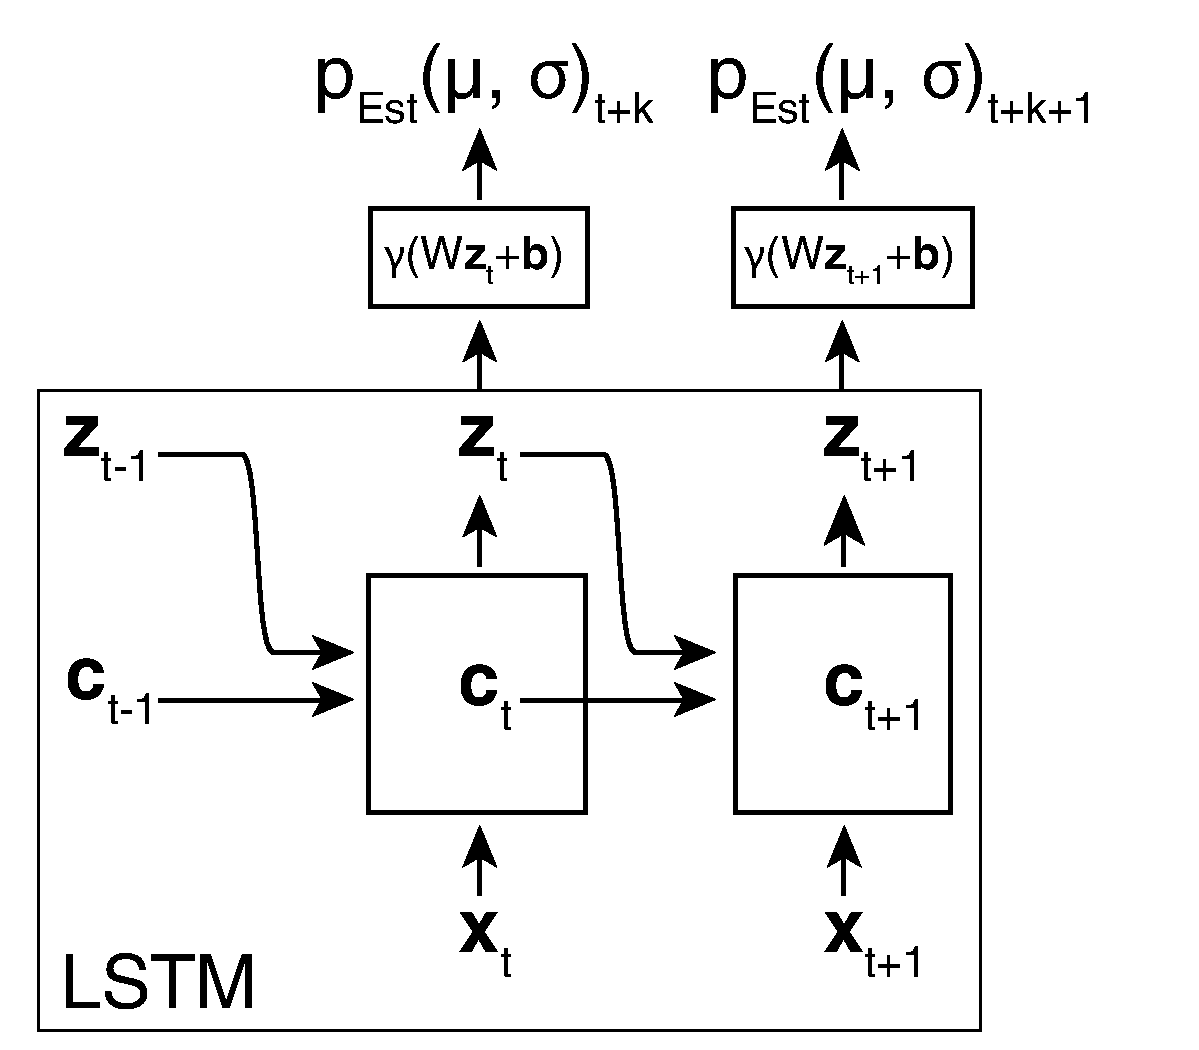
\includegraphics[width=0.7\textwidth]{figures/architecture_prob.pdf} % requires the graphicx package
   \caption{Schematic architecture for the deterministic network that learns parameters over an output distribution for Est. Our output distribution is a Gaussian. Two full time steps of network iteration are shown, with the portion of the network enclosing the LSTM cell labeled ``LSTM''.}
   \label{fig:architecture}
\end{figure}

We present an architecture (Figure~\ref{fig:architecture}) in which the NN learns to assess uncertainty in its own forecast, thereby generating probabilistic forecasts. The two basic layers utilized within this architecture are LSTM and dense layers. The former is described above, and the latter is an implementation of the so-called ``fully connected hidden layer'', which references the fact that each entry in $\mathbf{z}$ depends on all of the outputs from the preceding layer via $W$. That is, a dense layer that receives inputs $\mathbf{x} \in \mathbb{R}^n$ from a preceding network layer in turn generates an output vector $\mathbf{z} \in \mathbb{R}^m$ via the operation $\mathbf{z} = \gamma(W\,\mathbf{x} + \mathbf{b})$ with $W \in \mathbb{R}^{mxn}$ and $\mathbf{b} \in \mathbb{R}^m$, where $n$ is the dimensionality of the preceding hidden layer, $m$ is the dimensionality of the current hidden layer, and $\gamma(.)$ is a nonlinear activation function that acts element-wise. 

Inputs into our NN architecture are fed directly to an LSTM cell, and outputs from the LSTM cell are fed through a series of fully-connected hidden layers. The outputs from the last hidden layer are parameters for an output distribution over Est. We choose to use a Gaussian output distribution and compare other alternatives in the Supplement (Text S3). 

The simplest cost function in this probabilistic framework is precisely the output distribution itself evaluated as a likelihood of observed data $y$ (i.e., Est at some time $t+k$) with respect to the distribution parameters generated from the given input:
\begin{equation}
C(\mathbf{x}, y) = -\log p\left( y \vert \mu(W, \mathbf{b}, \mathbf{x}), \sigma(W, \mathbf{b}, \mathbf{x})\right) \label{eq:output}
\end{equation}
where the distribution parameters $\mu$ and $\sigma$ depend on the network weights and biases and can thus be differentiated against them. However, when learning two-parameter distributions, the parameter for scale often introduces leniency in the output distribution, allowing the network to expand uncertainty in its forecast rather than move its estimate for the center (see supplement Text S3). 

We found that utilizing a Gaussian output distribution with a regularized Gaussian likelihood as the cost function performed well for geomagnetic storm forecasting. Equation~\ref{eq:gaussian_mod} shows the form for this modified log-likelihood in which $\alpha\,(y-\mu)^2 + \beta\,\frac{1}{\sigma^2}$ are the terms that we have added, introducing $\alpha$ and $\beta$ as additional hyper-parameters. This regularization encourages the network to learn more reasonable estimates for $\mu$, offsetting the normalization by $\sigma^2$, while also allowing the user to further incentivize ($\beta > 0$) or penalize ($\beta < 0$) expanding forecast uncertainty.
\begin{equation}
    C_{\mathrm{Gaussian,\, regularized}}(y, \mu, \sigma) = \log\left(\sqrt{2\,\pi}\,\sigma \right) + \frac{\left(y-\mu \right)^2}{2\,\sigma^2} +  \alpha\,\left(y-\mu \right)^2 + \beta\,\frac{1}{\sigma^2} \label{eq:gaussian_mod}
\end{equation}
Other approaches have been formulated for learning uncertainty via neural networks, such as Bayes-by-Backprop \citep{Blundell2015}, which represents uncertainty in the network weights rather than in its output. Our implementation of this approach was not useful for storm forecasting (Supplement Text S2).

For all implementations, training, and testing of neural networks, we use Python wrappers for the learning framework TensorFlow \citep{tensorflow}. This framework is capable of representing neurons and the functional operations relating them as well as numerically computing the relevant gradients to train the network. TensorFlow provides an implementation of the high level deep learning Keras API (\url{https://keras.io/}), which allows for modular construction of networks from the layers described above. We also make use of the recently introduced TensorFlow Probability library, which provides a straightforward means of adding probability distributions as layers, allowing outputs from previous layers to be used as parameters for the distribution layers. These layers are compiled into a model that contains all the operations of the entire network as well as the particular cost functions and optimizers that dictate the learning process for given training inputs and outputs. We use the Adam optimizer for gradient update steps \citep{Kingma2014adam}. All neural network configuration and training parameters are listed in Supplement Text S4.


%%
%% OUTPUT DATA
%%
\subsection{Output Data}
Most geomagnetic storm forecasting thus far has emphasized prediction of Dst. However, Dst is actually a sum of internal and external components (Equation~\ref{eq:dst}), and the internal component, Ist, is generated by currents induced in Earth's subsurface by variation in the external component, Est \citep{Maus2004} \deleted{(Equation~4},
\begin{eqnarray}
    Dst(t) = Ist(t) + Est(t) \label{eq:dst}\\
    \textnormal{and}\nonumber \\
    Ist(t) = \int_{-\infty}^t Q(t-\tau)\,Est(\tau) d\tau \label{eq:ist},
\end{eqnarray}
where $Q(t-\tau)$ is the \deleted{induction kernel}\added{impulse response} that depends on \deleted{a radial}\added{subsurface} electrical conductivity \added{$\sigma$}\deleted{profile of subsurface}\added{, assuming that $\sigma \equiv \sigma(r)$ varies only along radial direction. This decomposition is easier to express in frequency domain, in which $Q(t)$ becomes the transfer function that relates internal and external components such that $\tilde{Ist}(\omega)=\tilde{Q}(\omega)\tilde{Est}(\omega)$. Subsequently, Est and Ist can be computed as \citep{Maus2004}:}
\begin{eqnarray}
    \added{\tilde{Est}(\omega) = \frac{1}{1+\tilde{Q}(\omega)}\,\tilde{Dst}(\omega)} \\
    \added{\tilde{Ist}(\omega) = \frac{\tilde{Q}(\omega)}{1+\tilde{Q}(\omega)}\,\tilde{Dst}(\omega)}
\end{eqnarray}
\added{with knowledge of $\tilde{Q}(\omega)$ and observations of Dst. For more details about this decomposition and the induction transfer functions, the reader is referred to} \cite{Maus2004, Olsen2005, Grayver2020}.

The problem of forecasting Dst is then actually two separate problems: the first is forecasting Est, and the second is learning Earth's induction response, Ist. With a suitable model of Earth's subsurface conductivity structure, however, knowledge of Est is sufficient to reconstruct Ist and thereby Dst. Furthermore, because the external field is what responds to magnetospheric activity anyway, it is more natural to forecast Est than Dst. Therefore, we generate forecasts of Est, and the data accessed from NOAA were generated following the methodology of \cite{Maus2004} \deleted{who utilize a one-dimensional conductivity model for the decomposition of Dst into Ist and Est}. 

This approach will be increasingly important as we attempt to forecast higher order structure in Earth's external field. Est captures only the first zonal (dipole) component of external magnetic field variability, but significant variation exists on shorter spatial scales, where the interaction with local conductivity structures becomes more important and complicated \citep{Kelbert2020}. Given that the ultimate goal of geomagnetic storm forecasting is to forecast GICs, it is important to note that GICs themselves depend strongly on local conductivity structures and local external magnetic field variability \citep{Olsen2004, Puethe2014}. The first step to forecasting these higher order external field coefficients is forecasting a single external field coefficient, Est, which is the focus of this work.


%%
%% DATA AND SOURCES
%%
\subsection{Input Data}

Two basic observation types relevant to geomagnetic storm forecasting have been made for the past few decades: the first includes measurements of the solar wind made in situ around the L1 point in the Earth-Sun system, and the second are measurements made directly of the solar disk and corona. These two data streams provide related but temporally disjoint information. Radiative phenomena on the solar disk take under nine minutes to be observed at Earth, while the solar wind requires two to five days to propagate from the solar disk to the L1 point. The L1 point is only 1.5$\times 10^{6}$~km from Earth, however, which is approximately one hour travel time at typical solar wind speeds (mean solar wind speed is roughly 440~km~s$^{-1}$ from the OMNI dataset).

Thus, while solar wind measurements near Earth's magnetosphere are ultimately the most relevant quantities for accurate geomagnetic storm forecasting, using only observations from the L1 point limits the forecast time to roughly an hour \citep{Shprits2019}. On the other hand, solar activity is ultimately responsible for all geomagnetic storms, but identifying which phenomena on the solar disk have the potential to cause geomagnetic storms and predicting the storm lag times and amplitudes resulting from those phenomena are not trivial tasks. Observations from the solar disk include measurements of coronal mass ejections (CMEs) around the perimeter of the disk, images of the solar surface at various wavelengths, and surface radiative fluxes. 

Input data come from three sources: the OMNI, GOES, and SOHO LASCO CME datasets. All details on data preprocessing are briefly discussed in the supplement (Text S2).

The low (hourly) resolution OMNI data include several solar wind and solar observations, which we extracted for the years 1995-2018. During this time interval, measurements of the solar wind (SW) come from the \added{WIND, IMP8, Geotail, and }ACE \deleted{and DSCVR} satellite missions \deleted{at the L1 point}. The quantities that we use as input data from this dataset are the three components of the interplanetary magnetic field in geocentric solar magnetospheric (GSM) coordinates, SW velocity, SW particle density, SW temperature, and SW longitude and latitude incident on Earth's magnetosphere. \added{Because the OMNI dataset contains observations from near-Earth (e.g., IMP8) and L1 (e.g., WIND, ACE) spacecraft, observations are propagated to the bow shock by adding time shifts that account for the spacecraft location and solar wind flow. These time shifts are included in the publicly available dataset, and we utilize the observation time stamps as they are reported.}

The GOES mission provided two time series of x-ray fluxes integrated over the solar disk. One series covered the wavelengths from 0.5-4~\r{A}, and the other series covered wavelengths 1-8~\r{A}. Given that these measurements vary over orders of magnitude, we take their logarithm as input. These data were reliably available from 1986 onwards.

The LASCO SOHO CME database provides a catalogue of CMEs observed around the perimeter of the solar disk, with five basic quantities estimated for each event: central position angle, angular width, speed, mass, and kinetic energy. Three estimates of speed are reported in the catalogue, all of which we include as training input. We only consider CMEs for which all data fields are reported, and during hours with multiple events, we take only the event with the largest estimated kinetic energy. The estimates of mass and kinetic energy varied over orders of magnitude, so we instead take their logarithms as input. The database contains measurements from 1996-2018.

\added{We did not attempt to time shift observations of the solar disk to the bow shock as is done for satellite observations at the L1 point in the OMNI dataset. This time lag between the solar disk and Earth's magnetosphere is precisely a learning problem of great interest that NN's may be able to help solve.}

Finally, previous observations of Est were included as input while forecasting future values. In total then data is available roughly from 1996 \replaced{through}{to} 2018. Of these 22 years, we take 18 years (approximately 158,000 hours) as training data, and 4 years for testing data (approximately 35,000 hours).


%%
%% EVALUATING NETWORK PERFORMANCE
%%
\subsection{Evaluating network performance}
In most geomagnetic storm forecasting to date, forecast accuracy is assessed by metrics such as the root mean square error and the Pearson correlation coefficient between forecasted and observed data. However, these statistics are generally not compared to those of a null hypothesis, for example persistence forecasting in which the best estimate for any time in the future is simply the last observed value. Due to the auto-correlative nature of the Est time series, persistence forecasting actually generates deceptively high correlations and low errors (\added{Figure~\ref{fig:skill},} Supplement Figure~S\replaced{9}{8}) \citep{Shprits2019}. In fact, all the networks in Supplement Table~S1 either underperform or barely outperform persistence forecasting as quantified by these two metrics. Furthermore, these metrics are computed over both quiet and disturbed times, while the ability to predict storms is the task of interest. Other than refining consideration of these metrics to only storm main phases, it is not obvious what metric best evaluates forecasting performance for models with deterministic output. 

With probabilistic networks, however, reliability curves provide a useful and easily interpretable metric to evaluate forecast performance. Each curve corresponds to a threshold in Est, and the axes compare the observed probability of exceeding that threshold compared to the predicted probability. A perfectly reliable forecast would generate curves that fall on the 1:1 line through the origin for all thresholds. If the observed reliability curve plots over the 1:1 line, then the forecast underestimates the occurrence of events exceeding that threshold, while if the reliability curve plots under the 1:1 line, the forecast is conservative and overestimates the occurrence of events exceeding the given threshold. Because these statistics are computed for thresholds in Est, the reliability assessment method by construction evaluates storm time forecasting separately from quiet time forecasting. We utilize reliability curves to assess forecast performance. 

Computing reliability curves requires binning data by intervals of predicted exceedance probabilities, which means that empirical statistics for infrequent, large storms will be less well constrained than smaller storms, particularly at large forecast probabilities. To assess uncertainty in the reliability curve computation, we use bootstrap resampling of forecasted and observed threshold exceedances to compute confidence intervals over observed threshold exceedances for a given bin of predicted threshold exceedance. Furthermore, we compute consistency intervals that indicate for the amount of data in each bin the spread in forecasting skill that one might anticipate from a perfectly reliable forecast \citep{Brocker2007}.
% LSTM
\subsection{Probabilistic Neural Network Architecture}
Recently, recurrent architectures for time series regression have emerged that combine ridge functions with state vectors to create units with ``memory''. The most successful of these has been the long short-term memory architecture (LSTM), introduced by \cite{Hochreiter1997}. The LSTM cell, as its name implies, uses new input data with both the previous output and previous internal state to update its internal state and generate new output (Supplement, Text S6). This architecture has been applied to Dst forecasting by \cite{Gruet2018}, but, like all previous applications of neural networks to storm forecasting (summarized in the Supplement, Table S1), the network generated deterministic output with no prediction of forecast uncertainty.

\begin{figure}[htbp]
   \centering
   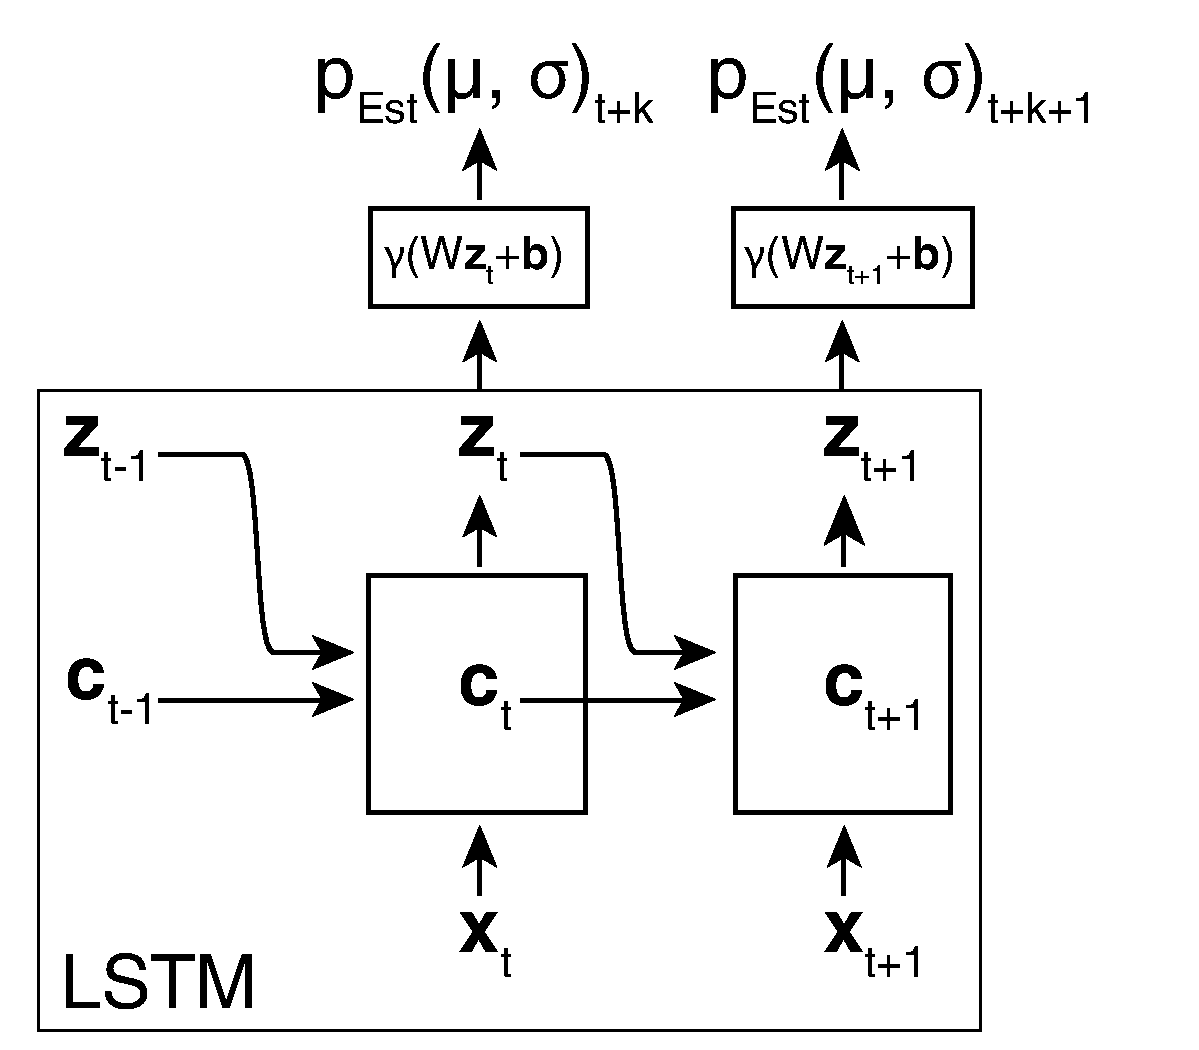
\includegraphics[width=0.7\textwidth]{figures/architecture_prob.pdf} % requires the graphicx package
   \caption{Schematic architecture for the deterministic network that learns parameters over an output distribution for Est. Our output distribution is a Gaussian. Two full time steps of network iteration are shown, with the portion of the network enclosing the LSTM cell labeled ``LSTM''.}
   \label{fig:architecture}
\end{figure}

We present an architecture (Figure~\ref{fig:architecture}) in which the NN learns to assess uncertainty in its own forecast, thereby generating probabilistic forecasts. The two basic layers utilized within this architecture are LSTM and dense layers. The former is described above, and the latter is an implementation of the so-called ``fully connected hidden layer'', which references the fact that each entry in $\mathbf{z}$ depends on all of the outputs from the preceding layer via $W$. That is, a dense layer that receives inputs $\mathbf{x} \in \mathbb{R}^n$ from a preceding network layer in turn generates an output vector $\mathbf{z} \in \mathbb{R}^m$ via the operation $\mathbf{z} = \gamma(W\,\mathbf{x} + \mathbf{b})$ with $W \in \mathbb{R}^{mxn}$ and $\mathbf{b} \in \mathbb{R}^m$, where $n$ is the dimensionality of the preceding hidden layer, $m$ is the dimensionality of the current hidden layer, and $\gamma(.)$ is a nonlinear activation function that acts element-wise. 

Inputs into our NN architecture are fed directly to an LSTM cell, and outputs from the LSTM cell are fed through a series of fully-connected hidden layers. The outputs from the last hidden layer are parameters for an output distribution over Est. We choose to use a Gaussian output distribution and compare other alternatives in the Supplement (Text S3). 

The simplest cost function in this probabilistic framework is precisely the output distribution itself evaluated as a likelihood of observed data $y$ (i.e., Est at some time $t+k$) with respect to the distribution parameters generated from the given input:
\begin{equation}
C(\mathbf{x}, y) = -\log p\left( y \vert \mu(W, \mathbf{b}, \mathbf{x}), \sigma(W, \mathbf{b}, \mathbf{x})\right) \label{eq:output}
\end{equation}
where the distribution parameters $\mu$ and $\sigma$ depend on the network weights and biases and can thus be differentiated against them. However, when learning two-parameter distributions, the parameter for scale often introduces leniency in the output distribution, allowing the network to expand uncertainty in its forecast rather than move its estimate for the center (see supplement Text S3). 

We found that utilizing a Gaussian output distribution with a regularized Gaussian likelihood as the cost function performed well for geomagnetic storm forecasting. Equation~\ref{eq:gaussian_mod} shows the form for this modified log-likelihood in which $\alpha\,(y-\mu)^2 + \beta\,\frac{1}{\sigma^2}$ are the terms that we have added, introducing $\alpha$ and $\beta$ as additional hyper-parameters. This regularization encourages the network to learn more reasonable estimates for $\mu$, offsetting the normalization by $\sigma^2$, while also allowing the user to further incentivize ($\beta > 0$) or penalize ($\beta < 0$) expanding forecast uncertainty.
\begin{equation}
    C_{\mathrm{Gaussian,\, regularized}}(y, \mu, \sigma) = \log\left(\sqrt{2\,\pi}\,\sigma \right) + \frac{\left(y-\mu \right)^2}{2\,\sigma^2} +  \alpha\,\left(y-\mu \right)^2 + \beta\,\frac{1}{\sigma^2} \label{eq:gaussian_mod}
\end{equation}
Other approaches have been formulated for learning uncertainty via neural networks, such as Bayes-by-Backprop \citep{Blundell2015}, which represents uncertainty in the network weights rather than in its output. Our implementation of this approach was not useful for storm forecasting (Supplement Text S2).

For all implementations, training, and testing of neural networks, we use Python wrappers for the learning framework TensorFlow \citep{tensorflow}. This framework is capable of representing neurons and the functional operations relating them as well as numerically computing the relevant gradients to train the network. TensorFlow provides an implementation of the high level deep learning Keras API (\url{https://keras.io/}), which allows for modular construction of networks from the layers described above. We also make use of the recently introduced TensorFlow Probability library, which provides a straightforward means of adding probability distributions as layers, allowing outputs from previous layers to be used as parameters for the distribution layers. These layers are compiled into a model that contains all the operations of the entire network as well as the particular cost functions and optimizers that dictate the learning process for given training inputs and outputs. We use the Adam optimizer for gradient update steps \citep{Kingma2014adam}. All neural network configuration and training parameters are listed in Supplement Text S4.


%%
%% OUTPUT DATA
%%
\subsection{Output Data}
Most geomagnetic storm forecasting thus far has emphasized prediction of Dst. However, Dst is actually a sum of internal and external components (Equation~\ref{eq:dst}), and the internal component, Ist, is generated by currents induced in Earth's subsurface by variation in the external component, Est \citep{Maus2004} \deleted{(Equation~4},
\begin{eqnarray}
    Dst(t) = Ist(t) + Est(t) \label{eq:dst}\\
    \textnormal{and}\nonumber \\
    Ist(t) = \int_{-\infty}^t Q(t-\tau)\,Est(\tau) d\tau \label{eq:ist},
\end{eqnarray}
where $Q(t-\tau)$ is the \deleted{induction kernel}\added{impulse response} that depends on \deleted{a radial}\added{subsurface} electrical conductivity \added{$\sigma$}\deleted{profile of subsurface}\added{, assuming that $\sigma \equiv \sigma(r)$ varies only along radial direction. This decomposition is easier to express in frequency domain, in which $Q(t)$ becomes the transfer function that relates internal and external components such that $\tilde{Ist}(\omega)=\tilde{Q}(\omega)\tilde{Est}(\omega)$. Subsequently, Est and Ist can be computed as \citep{Maus2004}:}
\begin{eqnarray}
    \added{\tilde{Est}(\omega) = \frac{1}{1+\tilde{Q}(\omega)}\,\tilde{Dst}(\omega)} \\
    \added{\tilde{Ist}(\omega) = \frac{\tilde{Q}(\omega)}{1+\tilde{Q}(\omega)}\,\tilde{Dst}(\omega)}
\end{eqnarray}
\added{with knowledge of $\tilde{Q}(\omega)$ and observations of Dst. For more details about this decomposition and the induction transfer functions, the reader is referred to} \cite{Maus2004, Olsen2005, Grayver2020}.

The problem of forecasting Dst is then actually two separate problems: the first is forecasting Est, and the second is learning Earth's induction response, Ist. With a suitable model of Earth's subsurface conductivity structure, however, knowledge of Est is sufficient to reconstruct Ist and thereby Dst. Furthermore, because the external field is what responds to magnetospheric activity anyway, it is more natural to forecast Est than Dst. Therefore, we generate forecasts of Est, and the data accessed from NOAA were generated following the methodology of \cite{Maus2004} \deleted{who utilize a one-dimensional conductivity model for the decomposition of Dst into Ist and Est}. 

This approach will be increasingly important as we attempt to forecast higher order structure in Earth's external field. Est captures only the first zonal (dipole) component of external magnetic field variability, but significant variation exists on shorter spatial scales, where the interaction with local conductivity structures becomes more important and complicated \citep{Kelbert2020}. Given that the ultimate goal of geomagnetic storm forecasting is to forecast GICs, it is important to note that GICs themselves depend strongly on local conductivity structures and local external magnetic field variability \citep{Olsen2004, Puethe2014}. The first step to forecasting these higher order external field coefficients is forecasting a single external field coefficient, Est, which is the focus of this work.


%%
%% DATA AND SOURCES
%%
\subsection{Input Data}

Two basic observation types relevant to geomagnetic storm forecasting have been made for the past few decades: the first includes measurements of the solar wind made in situ around the L1 point in the Earth-Sun system, and the second are measurements made directly of the solar disk and corona. These two data streams provide related but temporally disjoint information. Radiative phenomena on the solar disk take under nine minutes to be observed at Earth, while the solar wind requires two to five days to propagate from the solar disk to the L1 point. The L1 point is only 1.5$\times 10^{6}$~km from Earth, however, which is approximately one hour travel time at typical solar wind speeds (mean solar wind speed is roughly 440~km~s$^{-1}$ from the OMNI dataset).

Thus, while solar wind measurements near Earth's magnetosphere are ultimately the most relevant quantities for accurate geomagnetic storm forecasting, using only observations from the L1 point limits the forecast time to roughly an hour \citep{Shprits2019}. On the other hand, solar activity is ultimately responsible for all geomagnetic storms, but identifying which phenomena on the solar disk have the potential to cause geomagnetic storms and predicting the storm lag times and amplitudes resulting from those phenomena are not trivial tasks. Observations from the solar disk include measurements of coronal mass ejections (CMEs) around the perimeter of the disk, images of the solar surface at various wavelengths, and surface radiative fluxes. 

Input data come from three sources: the OMNI, GOES, and SOHO LASCO CME datasets. All details on data preprocessing are briefly discussed in the supplement (Text S2).

The low (hourly) resolution OMNI data include several solar wind and solar observations, which we extracted for the years 1995-2018. During this time interval, measurements of the solar wind (SW) come from the \added{WIND, IMP8, Geotail, and }ACE \deleted{and DSCVR} satellite missions \deleted{at the L1 point}. The quantities that we use as input data from this dataset are the three components of the interplanetary magnetic field in geocentric solar magnetospheric (GSM) coordinates, SW velocity, SW particle density, SW temperature, and SW longitude and latitude incident on Earth's magnetosphere. \added{Because the OMNI dataset contains observations from near-Earth (e.g., IMP8) and L1 (e.g., WIND, ACE) spacecraft, observations are propagated to the bow shock by adding time shifts that account for the spacecraft location and solar wind flow. These time shifts are included in the publicly available dataset, and we utilize the observation time stamps as they are reported.}

The GOES mission provided two time series of x-ray fluxes integrated over the solar disk. One series covered the wavelengths from 0.5-4~\r{A}, and the other series covered wavelengths 1-8~\r{A}. Given that these measurements vary over orders of magnitude, we take their logarithm as input. These data were reliably available from 1986 onwards.

The LASCO SOHO CME database provides a catalogue of CMEs observed around the perimeter of the solar disk, with five basic quantities estimated for each event: central position angle, angular width, speed, mass, and kinetic energy. Three estimates of speed are reported in the catalogue, all of which we include as training input. We only consider CMEs for which all data fields are reported, and during hours with multiple events, we take only the event with the largest estimated kinetic energy. The estimates of mass and kinetic energy varied over orders of magnitude, so we instead take their logarithms as input. The database contains measurements from 1996-2018.

\added{We did not attempt to time shift observations of the solar disk to the bow shock as is done for satellite observations at the L1 point in the OMNI dataset. This time lag between the solar disk and Earth's magnetosphere is precisely a learning problem of great interest that NN's may be able to help solve.}

Finally, previous observations of Est were included as input while forecasting future values. In total then data is available roughly from 1996 \replaced{through}{to} 2018. Of these 22 years, we take 18 years (approximately 158,000 hours) as training data, and 4 years for testing data (approximately 35,000 hours).


%%
%% EVALUATING NETWORK PERFORMANCE
%%
\subsection{Evaluating network performance}
In most geomagnetic storm forecasting to date, forecast accuracy is assessed by metrics such as the root mean square error and the Pearson correlation coefficient between forecasted and observed data. However, these statistics are generally not compared to those of a null hypothesis, for example persistence forecasting in which the best estimate for any time in the future is simply the last observed value. Due to the auto-correlative nature of the Est time series, persistence forecasting actually generates deceptively high correlations and low errors (\added{Figure~\ref{fig:skill},} Supplement Figure~S\replaced{9}{8}) \citep{Shprits2019}. In fact, all the networks in Supplement Table~S1 either underperform or barely outperform persistence forecasting as quantified by these two metrics. Furthermore, these metrics are computed over both quiet and disturbed times, while the ability to predict storms is the task of interest. Other than refining consideration of these metrics to only storm main phases, it is not obvious what metric best evaluates forecasting performance for models with deterministic output. 

With probabilistic networks, however, reliability curves provide a useful and easily interpretable metric to evaluate forecast performance. Each curve corresponds to a threshold in Est, and the axes compare the observed probability of exceeding that threshold compared to the predicted probability. A perfectly reliable forecast would generate curves that fall on the 1:1 line through the origin for all thresholds. If the observed reliability curve plots over the 1:1 line, then the forecast underestimates the occurrence of events exceeding that threshold, while if the reliability curve plots under the 1:1 line, the forecast is conservative and overestimates the occurrence of events exceeding the given threshold. Because these statistics are computed for thresholds in Est, the reliability assessment method by construction evaluates storm time forecasting separately from quiet time forecasting. We utilize reliability curves to assess forecast performance. 

Computing reliability curves requires binning data by intervals of predicted exceedance probabilities, which means that empirical statistics for infrequent, large storms will be less well constrained than smaller storms, particularly at large forecast probabilities. To assess uncertainty in the reliability curve computation, we use bootstrap resampling of forecasted and observed threshold exceedances to compute confidence intervals over observed threshold exceedances for a given bin of predicted threshold exceedance. Furthermore, we compute consistency intervals that indicate for the amount of data in each bin the spread in forecasting skill that one might anticipate from a perfectly reliable forecast \citep{Brocker2007}.

\section{Results and Discussion}
% In general, our architecture is capable of learning meaningful and reliable measures of uncertainty in its forecasts\added{, and our forecasts outperform the basic benchmark of persistence forecasting}. We \replaced{focus in our discussion on the}{discuss the architecture} performance \replaced{of the}{here by restricting ourselves to} six-hour ahead probabilistic forecasts \deleted{from the network trained with both L1 and solar disk inputs} \replaced{because this forecast window is long enough that information from the L1 point is insufficient to forecast storm arrivals, allowing us to evaluate whether our network is able to leverage information from the solar disk.}{for three different storms: two caused by CMEs (Figure 2A & B) and one resulting from a co-rotating interaction region (CIR) (Figure 2C). One to six hour ahead forecasts, as well as detailed comparison of the networks trained with only L1 data and both L1 and solar disk inputs, can be found in the Supplement.}  

% storm exmaples
\subsection{\added{Storm Case Studies}}
\added{We present and discuss in this section six hour ahead forecasts} for three different storms: two caused by CMEs (Figure~\ref{fig:storms}A \& B) and one resulting from a co-rotating interaction region (CIR) (Figure~\ref{fig:storms}C). One to six hour ahead forecasts, as well as detailed comparison of the networks trained with only L1 data and both L1 and solar disk inputs, can be found in the Supplement.

\begin{figure}[htbp]
  \centering
  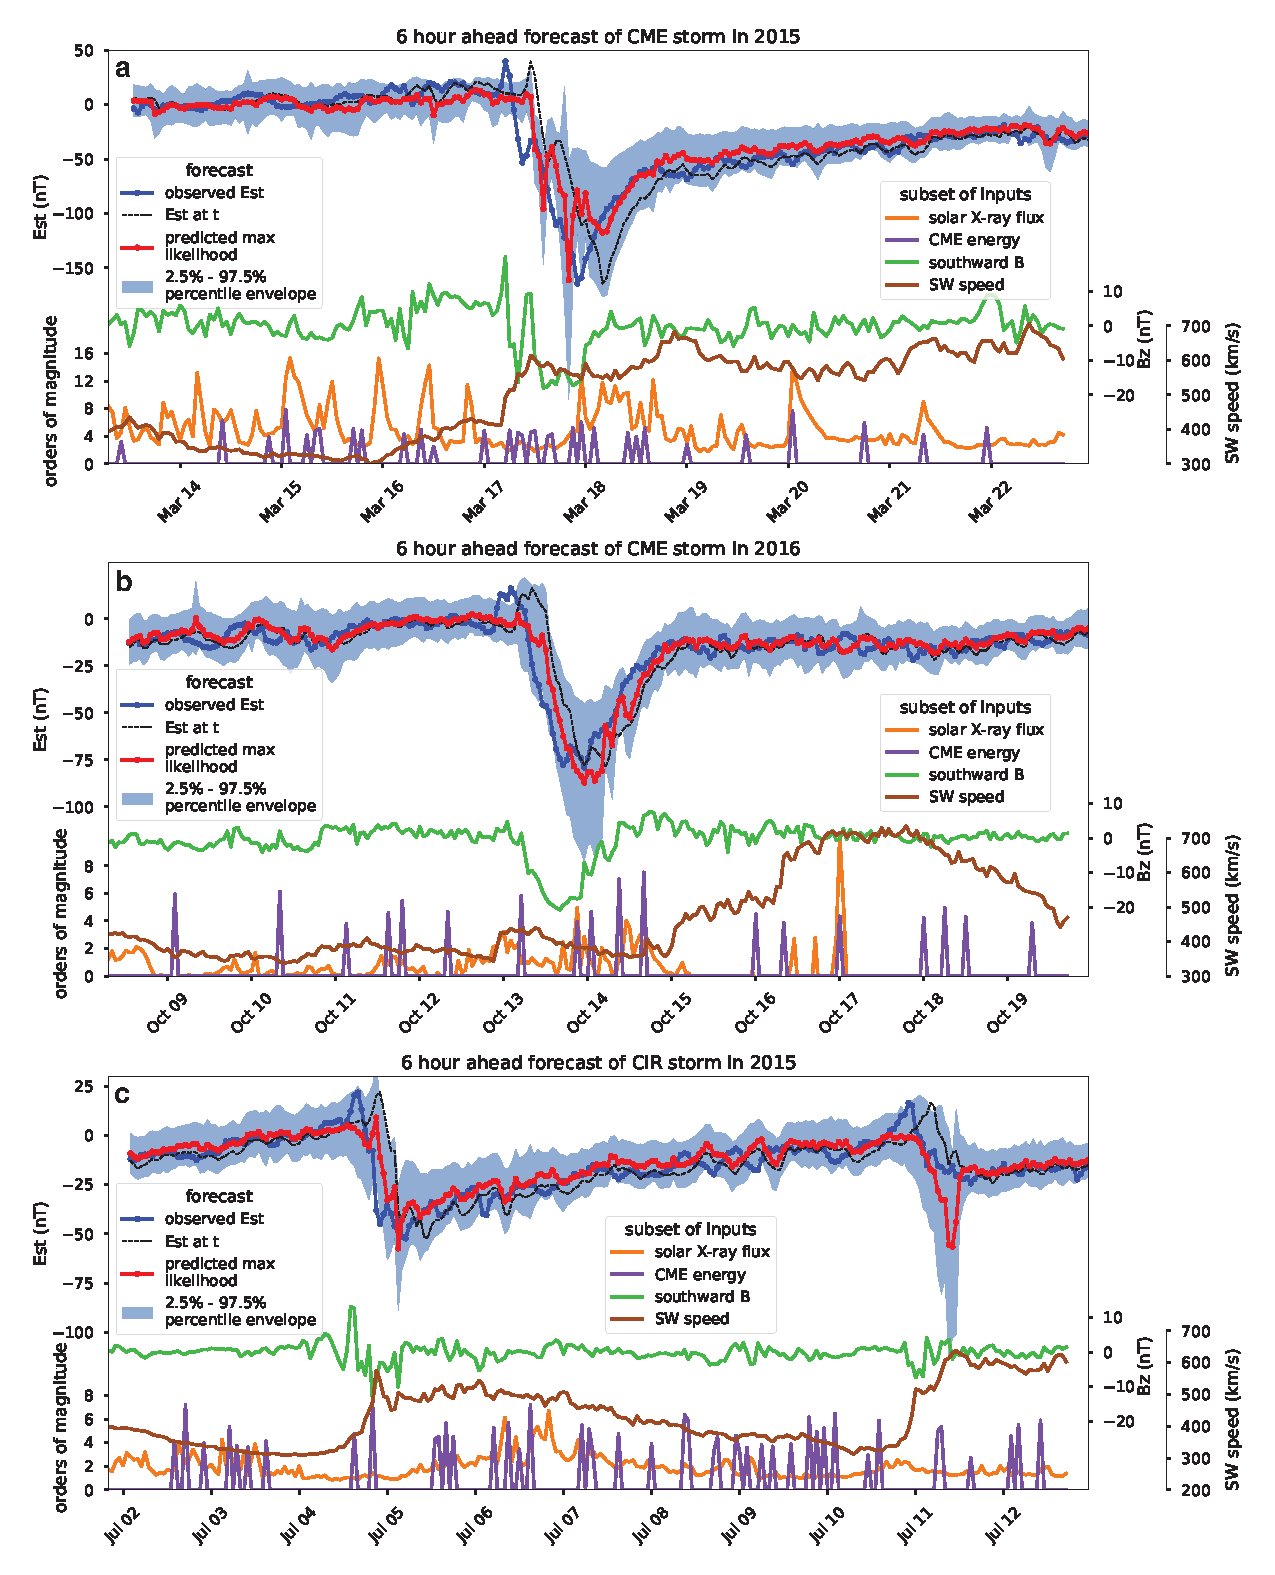
\includegraphics[width=1.0\textwidth]{figures/storms.pdf} 
  \caption{Six-hour-ahead probabilistic forecasts on testing data for two CME storms and one CIR storm, as identified by \cite{Patel2019, Shen2017}. Order of magnitude variability in x-ray flux (long channel is plotted) is exaggerated by ten times. The black dashed line for Est is a persistence forecast. \textbf{(a)} Severe CME geomagnetic storm (min Dst=-222~nT). Large amplitude variability in the southward component of the IMF might be responsible for forecast variability as the storm enters the main phase. \textbf{(b)} Intense CME geomagnetic storm (min Dst=-104~nT). \textbf{(c)} Intense CIR geomagnetic storm (min SYM-H=-87~nT). Order of magnitude variability in x-ray flux here is only exaggerated by five times.}
  \label{fig:storms}
\end{figure}

The first storm, in March of 2015, provides a prototypical example of a geomagnetic storm caused by a magnetic cloud emitted by the mass ejection visible as the spike in CME energy at the beginning of March 15 (Figure~\ref{fig:storms}A, note that the axis is orders of magnitude) \citep{Patel2019}. The energetic mass ejection is associated with a peak in integrated x-ray fluxes, followed two days later by a relatively large geomagnetic storm beginning on March 17. The storm main phase is associated with a sustained southward IMF of roughly -20~nT and roughly doubled solar wind speeds. In this situation, given the clear connection between the mass ejection and the ensuing storm, we would expect a successfully trained network to be able to expand uncertainty in its forecast as conceivable storm arrival times approach, reflecting an understanding of the causal association between activity on the solar disk and geomagnetic storms. Yet, forecast uncertainties only expand when disturbed solar wind reaches the L1 point. At that time, the network becomes aware of the storm arrival and adjusts its output by dropping Est forecasts and increasing forecast uncertainty (Figure~\ref{fig:storms}A). The same is true for the smaller amplitude CME storm of October 13, 2016 in Figure~\ref{fig:storms}B, where forecast uncertainty only grows as soon as the storm arrives at the L1 point. This storm is associated with the CME visible on October 10 \citep{Patel2019}, so the occurrence of other CMEs of similar magnitude (e.g. on October 9 and 11) demonstrates non-uniqueness that illustrates why the network struggles to identify geoeffective solar activity from the provided inputs.

The final storm on July 4, 2015 was chosen because it corresponds to a CIR \citep{Shen2017}, as evidenced by a lack of sustained, southward IMF, a step increase in solar wind velocity, and relatively low amplitude storm-time Est (Figure~\ref{fig:storms}C). The nature of CIR storms differs from those originating from CMEs \citep{Zhang2007}, so we sought to investigate if the forecast for CIR storms differs from that for CME storms. Again, for the storm on July 4, the network is unable to preemptively expand forecast uncertainties in response to information from solar disk, demonstrating that inputs from the L1 point dominate the forecast. On July 11, the network mistakenly forecasts a storm main phase, likely in response to the increased solar wind speed that did not actually generate a substantial main phase.

% forecasting skill
In all cases, \replaced{the six hour ahead forecast fails to capture}{forecasting geomagnetic} storm onset\replaced{, during which the network's forecasts tend to lag observations by the forecast length (thereby more closely tracking the persistence curve) until the storm arrives at the L1 point. At that point, the forecast begins to deviate from persistence as the network knows that a storm is occurring. This inability to predict storm onset indicates that the network is unable to utilize observations from the solar disk for storm arrival, which remains an open challenge.}{is not improved by utilizing observational inputs from the solar disk.} 

\replaced{R}{but r}ecovery is generally well-predicted, and forecasts deviate from persistence, meaning that the network is not just taking the last observed Est value for its next forecast. Unlike previous results, our network is capable of generating meaningful estimates of uncertainty in its forecasts. In all cases, once the network detects the possible onset of a geomagnetic storm, it expands its forecast uncertainty, generally maintaining observed Est values within the 95\% forecast confidence interval and providing reliable multiple hour ahead forecasts (see Supplement Text S5 for one to six hour ahead forecasts). After storm main phases, forecast uncertainties decrease during the generally well-predicted recovery phase. Given that the recovery phase is dictated by the internal dynamics of the ring current decay (and thereby independent of the solar wind state) \citep{Daglis2007}, its predictability is reasonable. Thus, our network exhibits forecast uncertainties that are consistent with where one would anticipate the greatest uncertainty in geomagnetic storm development with information from the L1 point, namely, the storm onset and main phase.

% forecasting skill, conventional metrics
\subsection{\added{Conventional Metrics of Forecast Skill}}

\added{In terms of the conventional forecasting skill assessments (i.e., forecast-observation Pearson correlation coefficients and root-mean-square errors, RMSE's) for one to six hour ahead forecasts, our networks outperform all previous neural network forecasts for all forecasts lengths (Figure~\ref{fig:skill}). However, given that persistence forecasting for Est results in higher correlation coefficients and lower RMSE's than for persistence forecasting of Dst, our improvements should not be compared with previous results for forecasting Dst but with persistence forecasting of Est. When considering all observations, we slightly underperform persistence forecasting of Est in terms of the correlation coefficient, while outperforming in terms of RMSE, which is consistently lower. During storm times, however, our forecasting skill is much better than persistence forecasting in both metrics at all forecasting windows. The networks with both L1 and solar disk inputs always outperform networks with only L1 inputs when evaluated over both quiet and storm times (Figure S9). However, the difference in skill is small, and when considering only storm times, the five to six hour ahead forecasts of networks with only L1 inputs achieve lower RMSE's. These results again indicate that information from the solar disk does not significantly improve storm forecast skill. Finally, for particularly large storms exceeding Est $\leq$ -200~nT, a forecast saturation effect is observed (Figure S9), similar to that that occurs at smaller values with different cost functions (Supplement Text S3). This effect can be partially mitigated by fine-tuning of the cost function to further facilitate the forecasting of rare storms. However, since there is only a handful of such events in the data, this behaviour of the network is natural.}

\begin{figure}[htbp]
  \centering
  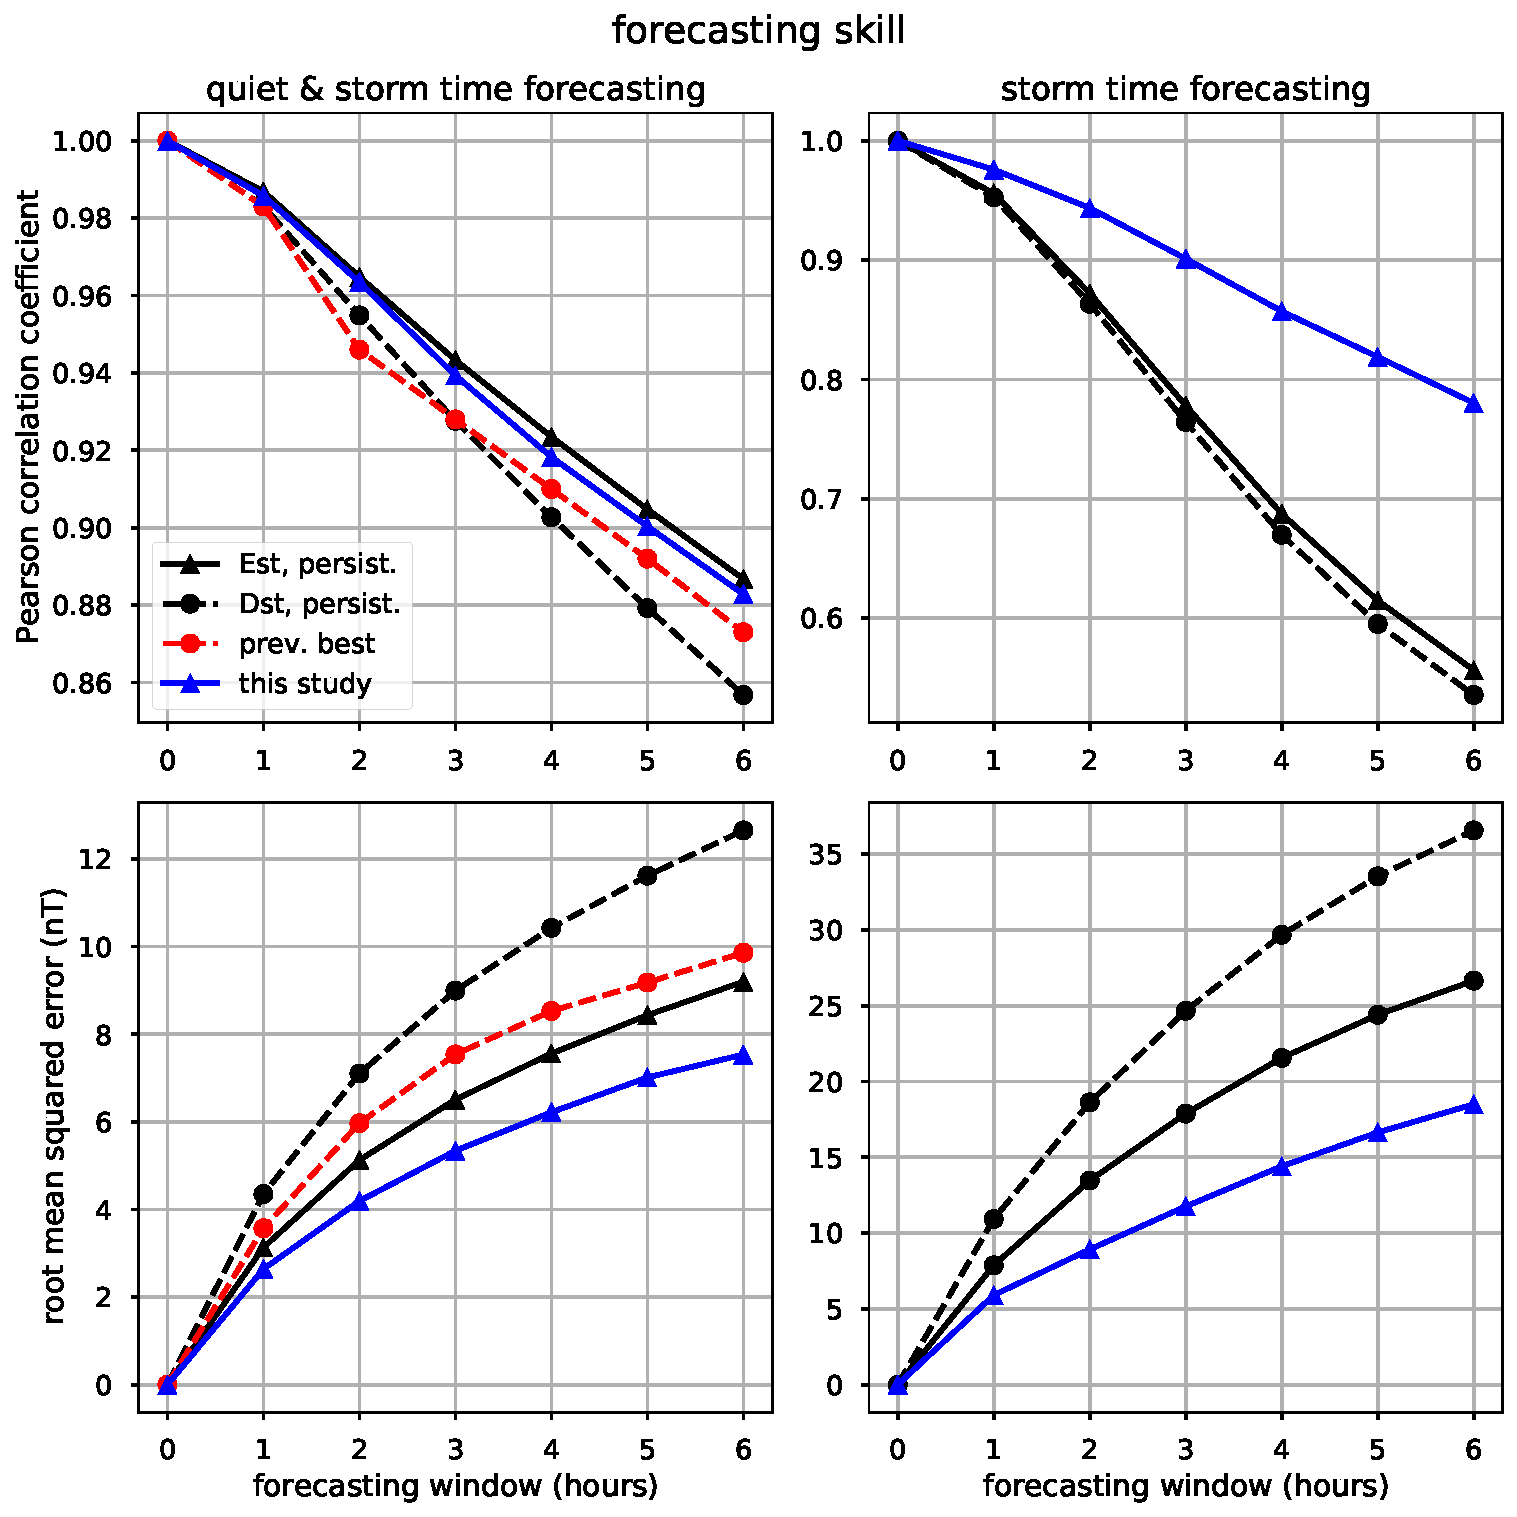
\includegraphics[width=1.0\textwidth]{figures/skill_comparison.pdf} 
  \caption{\added{Conventional metrics of forecasting skill for networks with both solar disk and L1 inputs (see Figure S9 for networks with only L1 inputs). The first row shows the Pearson correlation coefficient between the forecasted Est (mean, for our study) or Dst and the observed Est or Dst. The second row shows the corresponding root mean squared errors. In the columns, we show these quantities for all observations (first column) and only storm-time observations (second column). The black lines show the metrics for persistence forecasts of Est and Dst, and the red line (available only for all observations) shows the best reported performance from NN forecasts (see Table S1 for references).}}
  \label{fig:skill}
\end{figure}


% forecast reliability
\subsection{\added{Forecast Reliability}}

Reliabilities for four different storm thresholds generally overlap with the consistency intervals for each bin, demonstrating that our network generates reliable forecasts (Figure~\ref{fig:reliability}). For threshold of -75 and -100~nT, forecasted exceedance probabilities in the range of 0.7-0.9 tended to slightly underestimate observed exceedance rates, which is consistent with the observation that storm onsets remain difficult to predict exactly.

% adjust wording here
Notably, the regularization of the cost function for a Gaussian output distribution significantly improves forecast reliability. Networks trained with unregularized Gaussian and Gumbel output distributions (Supplement Text S3) are unable move the location parameters of their forecasts during large amplitude storms, preferring instead to expand forecast uncertainty, meaning that peak storm times, while often within the 95\% confidence interval, are only predicted at extremely low exceedance probabilities. This behavior explains why the reliability curves lack data to bin at high forecast probabilities and furthermore why storms are underestimated for lower exceedance probabilities (Figure~\ref{fig:reliability}).

\begin{figure}[htbp]
  \centering
  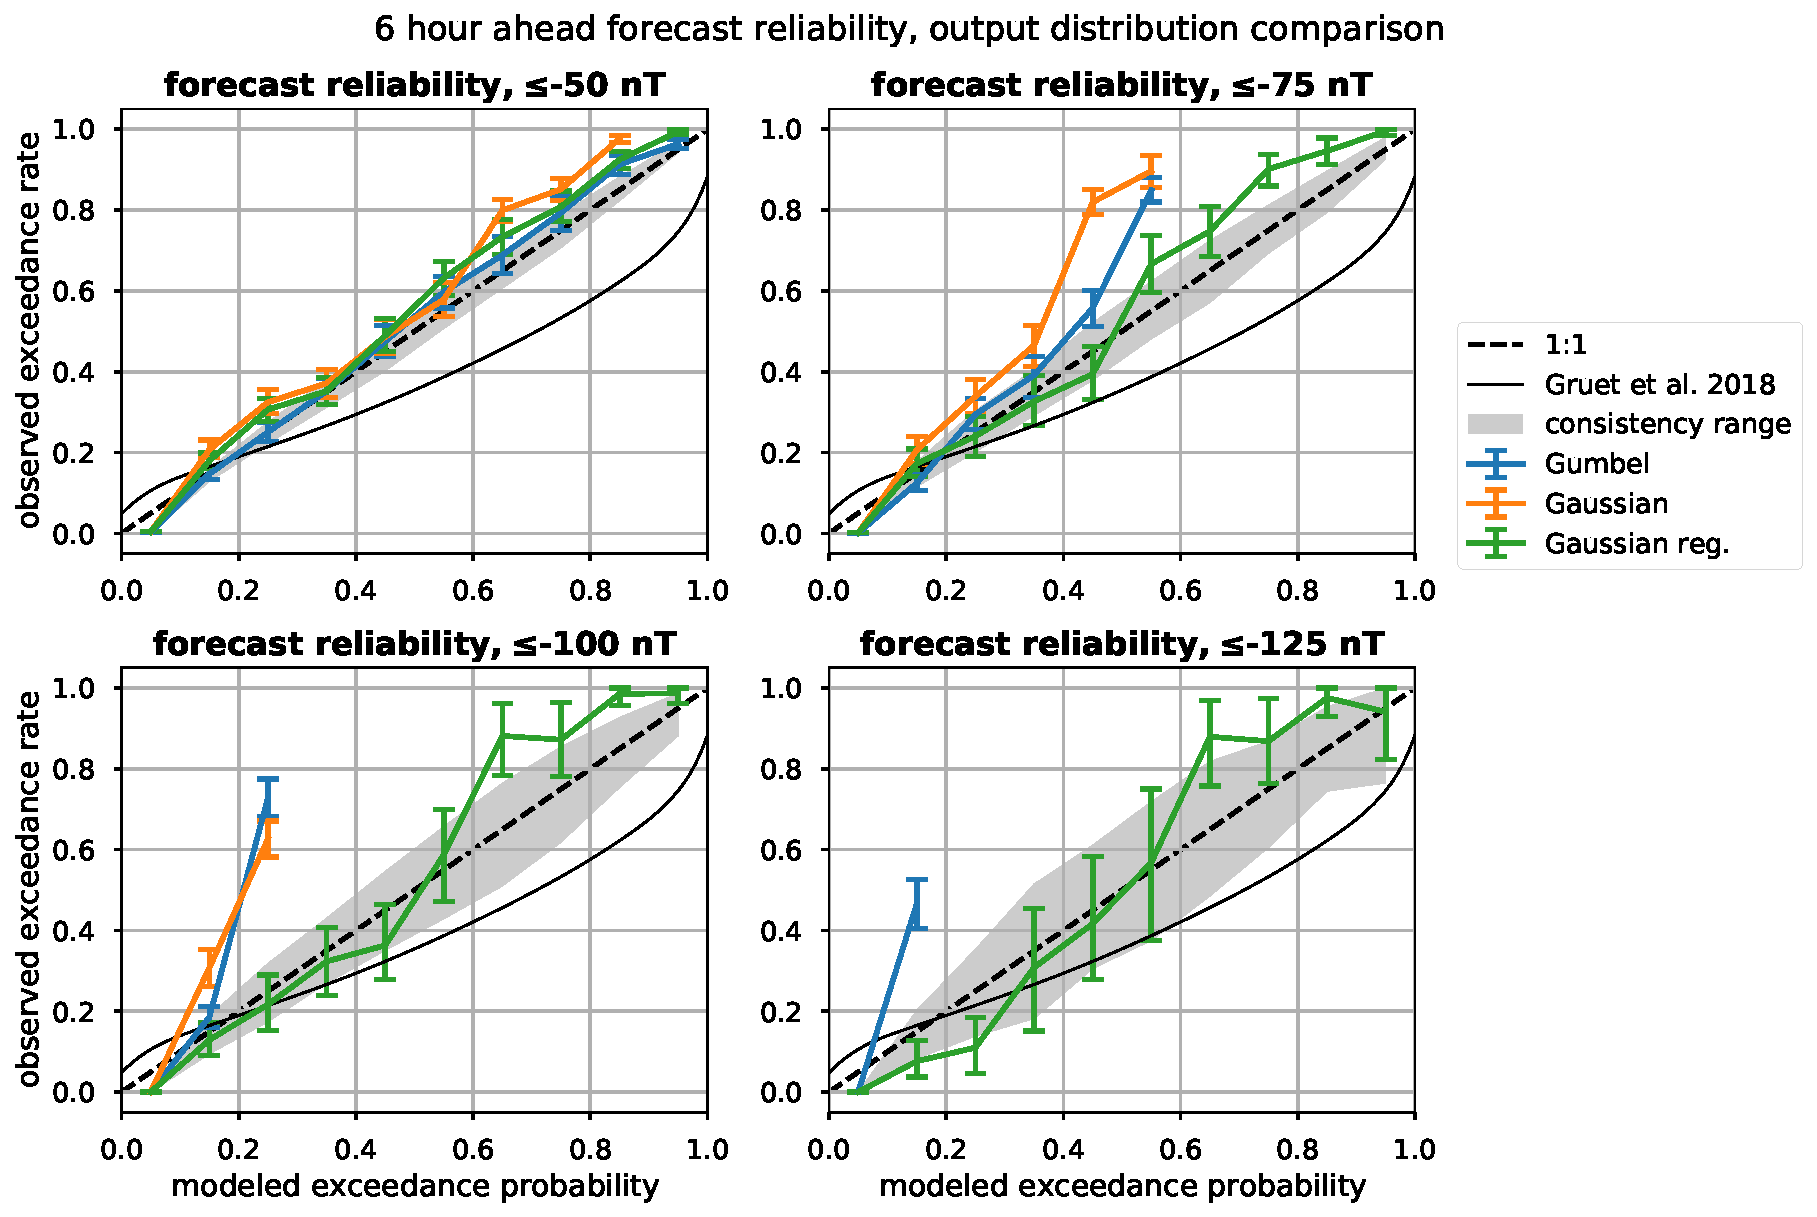
\includegraphics[width=1.0\textwidth]{figures/est_forecast_reliability_distcompare_t+6.pdf} 
  \caption{Reliability curves for the networks with a Gumbel output and cost (blue), Gaussian output and cost (orange), and Gaussian output with regularized cost (green). All curves are for a six hour ahead forecast for four Est thresholds in eleven bins. Exceedance was taken in the negative sense, i.e., taking values less than or equal to the given threshold. Error bars show the 2.5-97.5 percentile range from bootstrapped resampling (number of bootstrapped samples was 1000) within the bins of forecasted exceedance probability. The envelopes show the 2.5-97.5 percentile range from consistency resampling of a perfectly reliable forecast, demonstrating the conceivable range in reliable forecasts given the number of data in each bin \citep{Brocker2007}. The regularized Gaussian network is the most reliable of the three. \added{Also shown is the reliability curve from \cite{Gruet2018} for their six hour ahead Dst forecast, for which the exceedance threshold is unspecified.}}
  \label{fig:reliability}
\end{figure}

While some improvement in forecast reliability for smaller magnitude storms (Est thresholds of -50 and -75~nT) does seem to result from the incorporation of data from the solar disk (Supplement Figure S7), the preceding discussion and the result that forecast behavior does not qualitatively change by adding solar disk inputs (Supplement Text S5) indicates that we are unable to successfully utilize observations from the solar disk to forecast storm arrival and amplitude. This shortcoming suggests that the information necessary for identifying geoeffective solar activity is lacking in the training data, and/or that the network architecture is inadequate for utilizing these data. For instance, the x-ray fluxes are integrated over the entire solar disk, but peaks in these fluxes can often be associated with flare events, which themselves often occur simultaneously with geoeffective mass ejections \citep{Tobiska2013}. Larger, more central flares are associated with larger geomagnetic storms, so adding time series of flare occurrences with locations on the solar disk would complement the input series of x-ray fluxes and CMEs \citep{Tobiska2013}. Futhermore, the CME dataset only includes ejections visible around the rim of the solar disk, while geoeffective ejections occur towards the center. Thus, only centralized ejections that also emit an observable lobe beyond the rim of the solar disk could be reliably associated with geomagnetic storms, potentially rendering the CME database largely irrelevant for the problem of geomagnetic storm forecasting. Finally, integrated solar x-ray flux peaks from flares have been empirically related to solar wind speeds and geomagnetic storm amplitudes, thereby providing a means of learning lag times between solar activity and storm arrivals \citep{Tobiska2013}. However, LSTM networks struggle with learning lag times \citep{Gers2002}, so the network architecture we have utilized is not amenable to this task.  
In general, our architecture is capable of learning meaningful and reliable measures of uncertainty in its forecasts\added{, and our forecasts outperform the basic benchmark of persistence forecasting}. We \replaced{focus in our discussion on the}{discuss the architecture} performance \replaced{of the}{here by restricting ourselves to} six-hour ahead probabilistic forecasts \deleted{from the network trained with both L1 and solar disk inputs} \replaced{because this forecast window is long enough that information from the L1 point is insufficient to forecast storm arrivals, allowing us to evaluate whether our network is able to leverage information from the solar disk.}{for three different storms: two caused by CMEs (Figure 2A & B) and one resulting from a co-rotating interaction region (CIR) (Figure 2C). One to six hour ahead forecasts, as well as detailed comparison of the networks trained with only L1 data and both L1 and solar disk inputs, can be found in the Supplement.}  

% storm exmaples
\subsection{\added{Storm Case Studies}}
\added{We present and discuss in this section six hour ahead forecasts} for three different storms: two caused by CMEs (Figure~\ref{fig:storms}A \& B) and one resulting from a co-rotating interaction region (CIR) (Figure~\ref{fig:storms}C). One to six hour ahead forecasts, as well as detailed comparison of the networks trained with only L1 data and both L1 and solar disk inputs, can be found in the Supplement.

\begin{figure}[htbp]
  \centering
  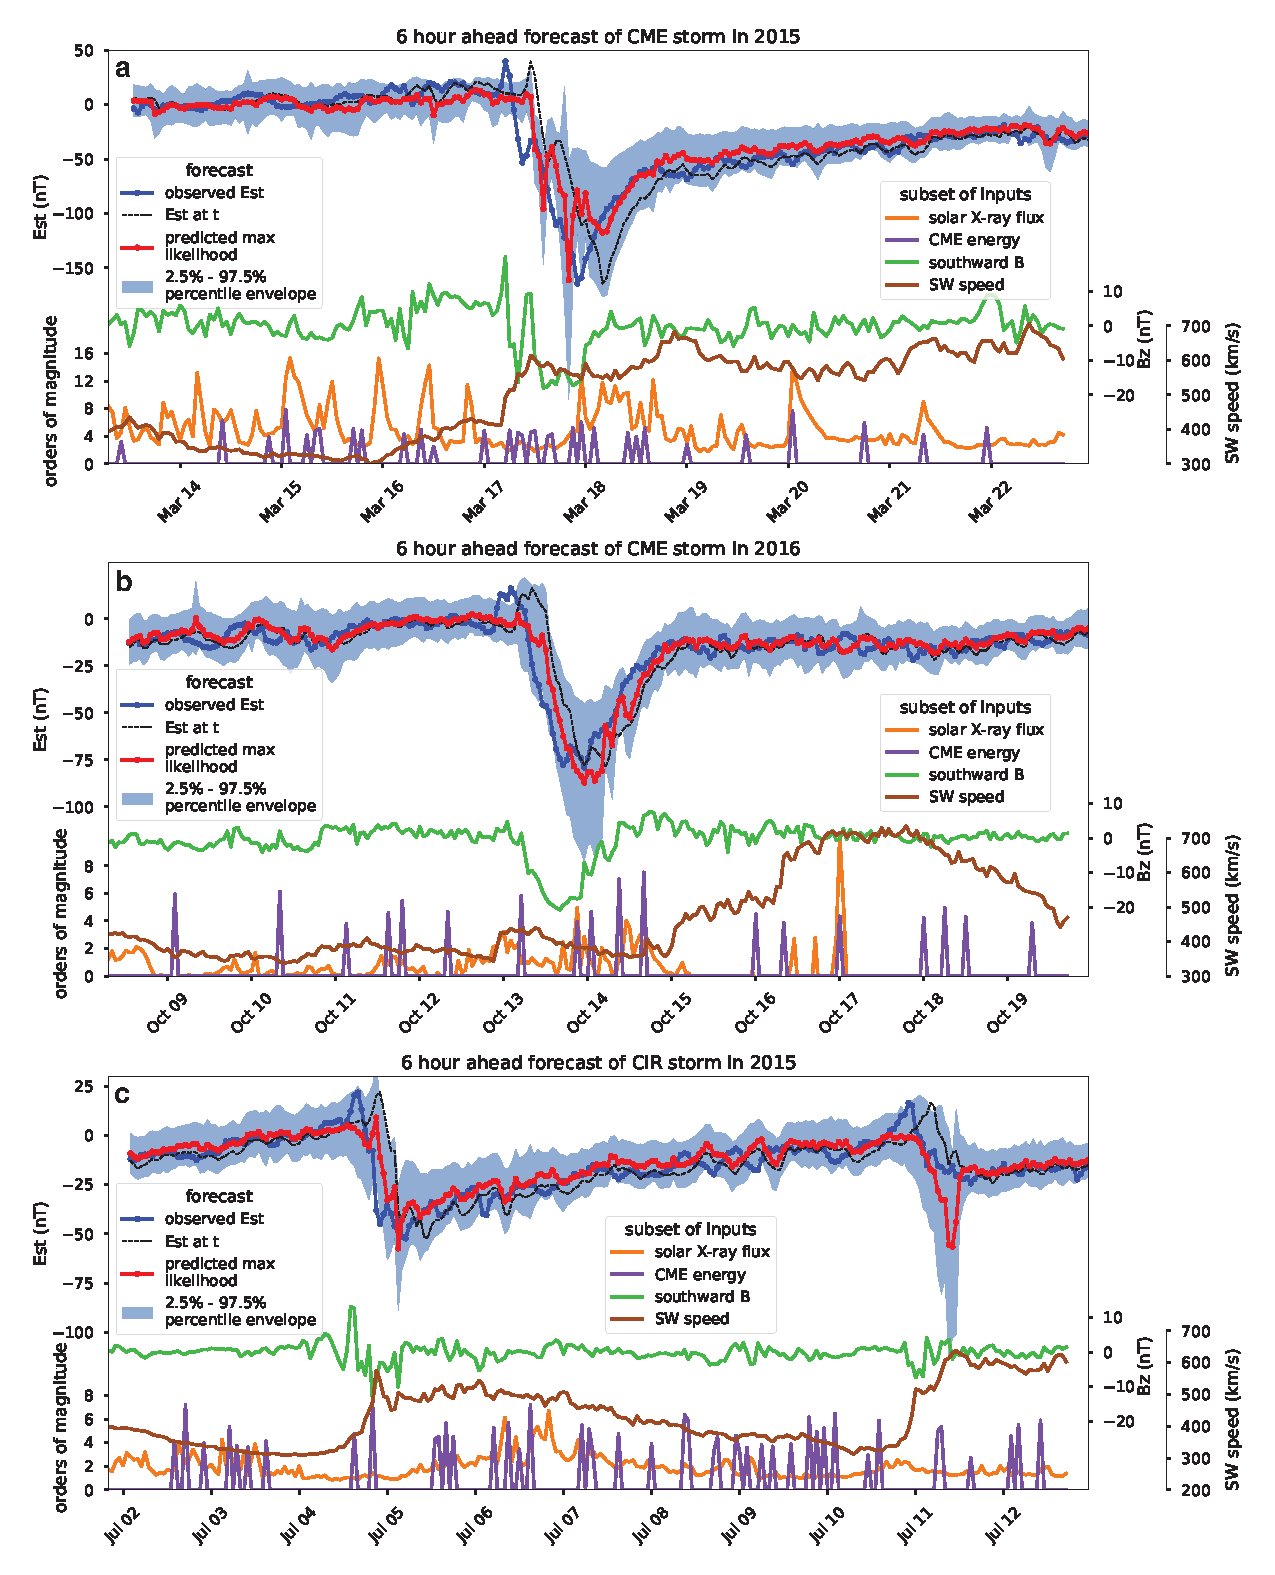
\includegraphics[width=1.0\textwidth]{figures/storms.pdf} 
  \caption{Six-hour-ahead probabilistic forecasts on testing data for two CME storms and one CIR storm, as identified by \cite{Patel2019, Shen2017}. Order of magnitude variability in x-ray flux (long channel is plotted) is exaggerated by ten times. The black dashed line for Est is a persistence forecast. \textbf{(a)} Severe CME geomagnetic storm (min Dst=-222~nT). Large amplitude variability in the southward component of the IMF might be responsible for forecast variability as the storm enters the main phase. \textbf{(b)} Intense CME geomagnetic storm (min Dst=-104~nT). \textbf{(c)} Intense CIR geomagnetic storm (min SYM-H=-87~nT). Order of magnitude variability in x-ray flux here is only exaggerated by five times.}
  \label{fig:storms}
\end{figure}

The first storm, in March of 2015, provides a prototypical example of a geomagnetic storm caused by a magnetic cloud emitted by the mass ejection visible as the spike in CME energy at the beginning of March 15 (Figure~\ref{fig:storms}A, note that the axis is orders of magnitude) \citep{Patel2019}. The energetic mass ejection is associated with a peak in integrated x-ray fluxes, followed two days later by a relatively large geomagnetic storm beginning on March 17. The storm main phase is associated with a sustained southward IMF of roughly -20~nT and roughly doubled solar wind speeds. In this situation, given the clear connection between the mass ejection and the ensuing storm, we would expect a successfully trained network to be able to expand uncertainty in its forecast as conceivable storm arrival times approach, reflecting an understanding of the causal association between activity on the solar disk and geomagnetic storms. Yet, forecast uncertainties only expand when disturbed solar wind reaches the L1 point. At that time, the network becomes aware of the storm arrival and adjusts its output by dropping Est forecasts and increasing forecast uncertainty (Figure~\ref{fig:storms}A). The same is true for the smaller amplitude CME storm of October 13, 2016 in Figure~\ref{fig:storms}B, where forecast uncertainty only grows as soon as the storm arrives at the L1 point. This storm is associated with the CME visible on October 10 \citep{Patel2019}, so the occurrence of other CMEs of similar magnitude (e.g. on October 9 and 11) demonstrates non-uniqueness that illustrates why the network struggles to identify geoeffective solar activity from the provided inputs.

The final storm on July 4, 2015 was chosen because it corresponds to a CIR \citep{Shen2017}, as evidenced by a lack of sustained, southward IMF, a step increase in solar wind velocity, and relatively low amplitude storm-time Est (Figure~\ref{fig:storms}C). The nature of CIR storms differs from those originating from CMEs \citep{Zhang2007}, so we sought to investigate if the forecast for CIR storms differs from that for CME storms. Again, for the storm on July 4, the network is unable to preemptively expand forecast uncertainties in response to information from solar disk, demonstrating that inputs from the L1 point dominate the forecast. On July 11, the network mistakenly forecasts a storm main phase, likely in response to the increased solar wind speed that did not actually generate a substantial main phase.

% forecasting skill
In all cases, \replaced{the six hour ahead forecast fails to capture}{forecasting geomagnetic} storm onset\replaced{, during which the network's forecasts tend to lag observations by the forecast length (thereby more closely tracking the persistence curve) until the storm arrives at the L1 point. At that point, the forecast begins to deviate from persistence as the network knows that a storm is occurring. This inability to predict storm onset indicates that the network is unable to utilize observations from the solar disk for storm arrival, which remains an open challenge.}{is not improved by utilizing observational inputs from the solar disk.} 

\replaced{R}{but r}ecovery is generally well-predicted, and forecasts deviate from persistence, meaning that the network is not just taking the last observed Est value for its next forecast. Unlike previous results, our network is capable of generating meaningful estimates of uncertainty in its forecasts. In all cases, once the network detects the possible onset of a geomagnetic storm, it expands its forecast uncertainty, generally maintaining observed Est values within the 95\% forecast confidence interval and providing reliable multiple hour ahead forecasts (see Supplement Text S5 for one to six hour ahead forecasts). After storm main phases, forecast uncertainties decrease during the generally well-predicted recovery phase. Given that the recovery phase is dictated by the internal dynamics of the ring current decay (and thereby independent of the solar wind state) \citep{Daglis2007}, its predictability is reasonable. Thus, our network exhibits forecast uncertainties that are consistent with where one would anticipate the greatest uncertainty in geomagnetic storm development with information from the L1 point, namely, the storm onset and main phase.

% forecasting skill, conventional metrics
\subsection{\added{Conventional Metrics of Forecast Skill}}

\added{In terms of the conventional forecasting skill assessments (i.e., forecast-observation Pearson correlation coefficients and root-mean-square errors, RMSE's) for one to six hour ahead forecasts, our networks outperform all previous neural network forecasts for all forecasts lengths (Figure~\ref{fig:skill}). However, given that persistence forecasting for Est results in higher correlation coefficients and lower RMSE's than for persistence forecasting of Dst, our improvements should not be compared with previous results for forecasting Dst but with persistence forecasting of Est. When considering all observations, we slightly underperform persistence forecasting of Est in terms of the correlation coefficient, while outperforming in terms of RMSE, which is consistently lower. During storm times, however, our forecasting skill is much better than persistence forecasting in both metrics at all forecasting windows. The networks with both L1 and solar disk inputs always outperform networks with only L1 inputs when evaluated over both quiet and storm times (Figure S9). However, the difference in skill is small, and when considering only storm times, the five to six hour ahead forecasts of networks with only L1 inputs achieve lower RMSE's. These results again indicate that information from the solar disk does not significantly improve storm forecast skill. Finally, for particularly large storms exceeding Est $\leq$ -200~nT, a forecast saturation effect is observed (Figure S9), similar to that that occurs at smaller values with different cost functions (Supplement Text S3). This effect can be partially mitigated by fine-tuning of the cost function to further facilitate the forecasting of rare storms. However, since there is only a handful of such events in the data, this behaviour of the network is natural.}

\begin{figure}[htbp]
  \centering
  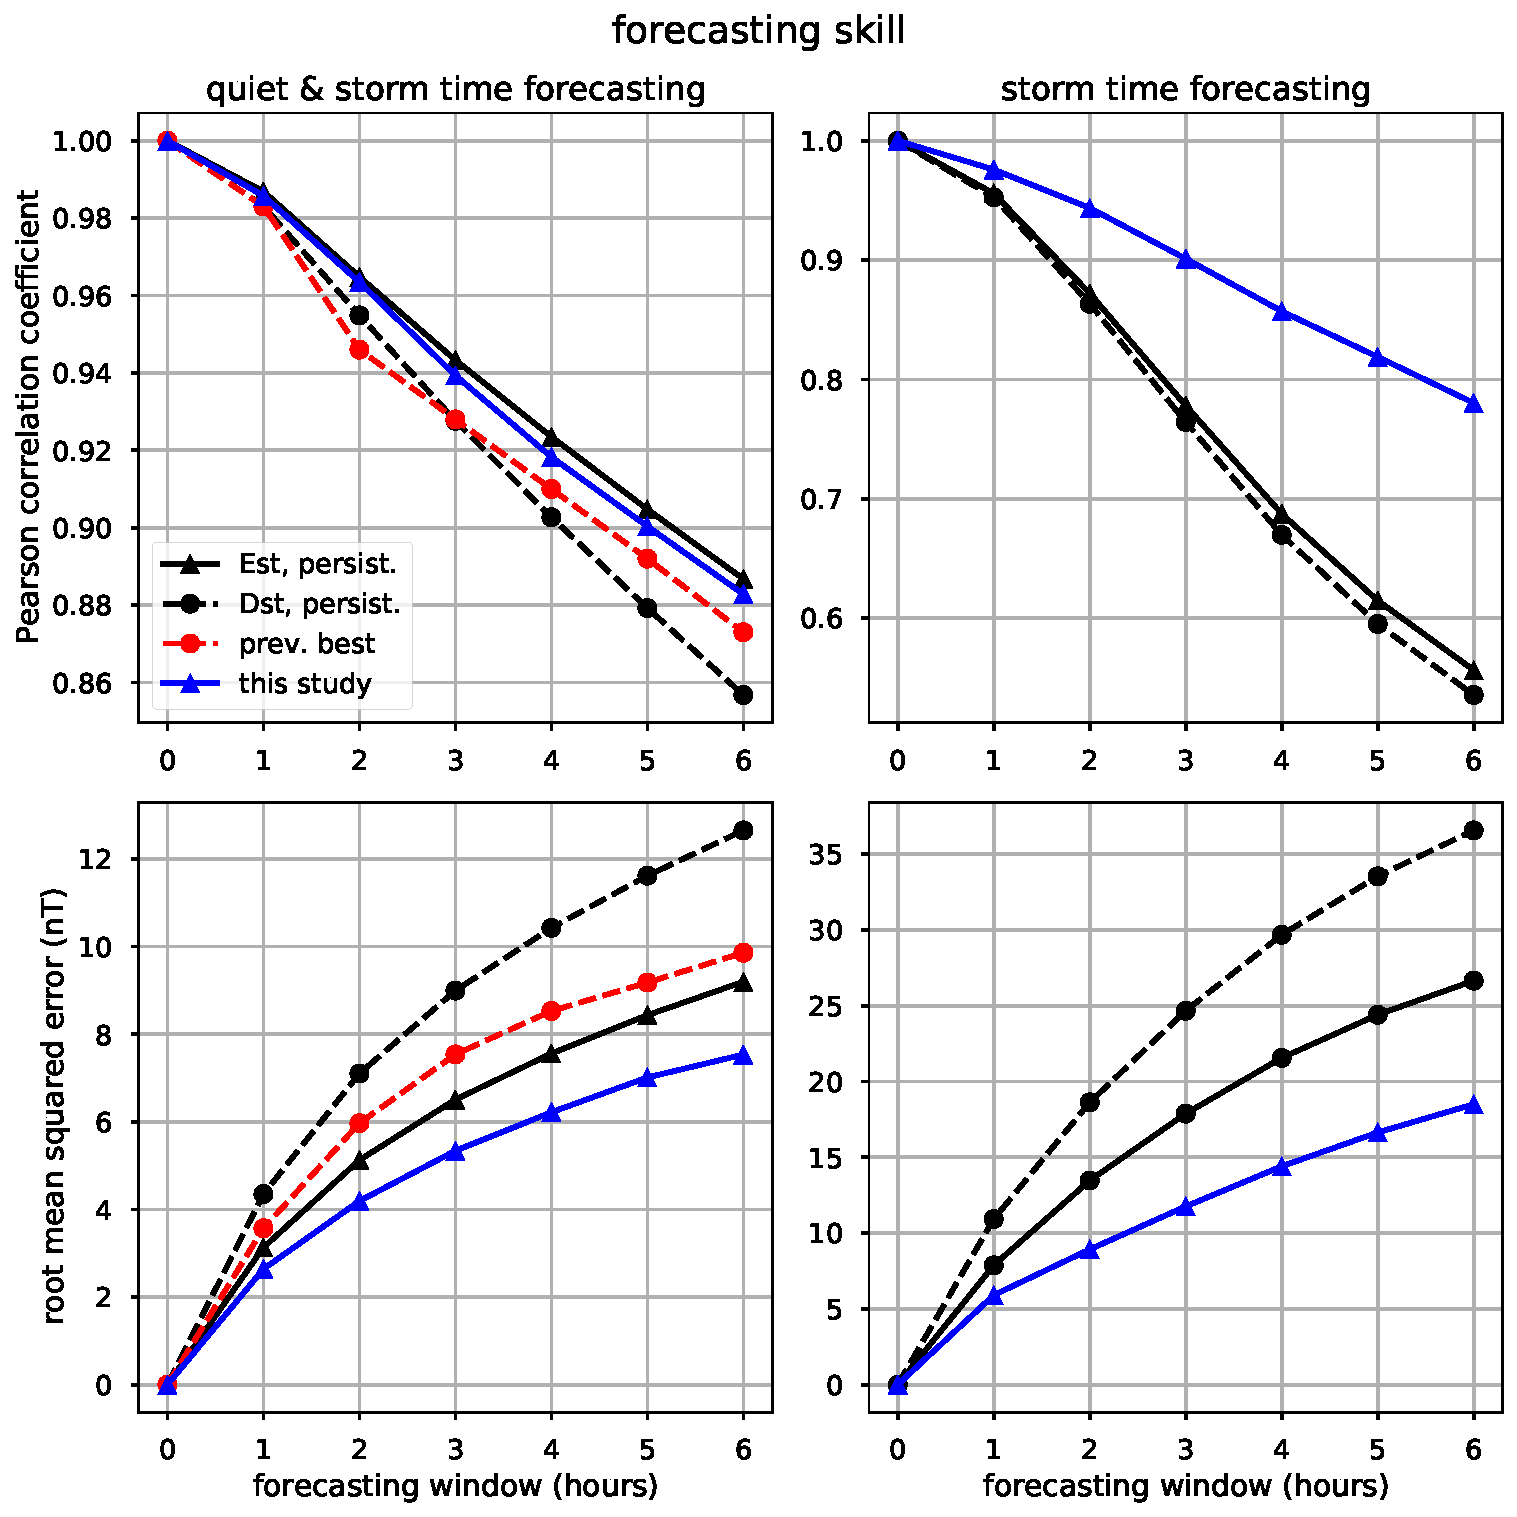
\includegraphics[width=1.0\textwidth]{figures/skill_comparison.pdf} 
  \caption{\added{Conventional metrics of forecasting skill for networks with both solar disk and L1 inputs (see Figure S9 for networks with only L1 inputs). The first row shows the Pearson correlation coefficient between the forecasted Est (mean, for our study) or Dst and the observed Est or Dst. The second row shows the corresponding root mean squared errors. In the columns, we show these quantities for all observations (first column) and only storm-time observations (second column). The black lines show the metrics for persistence forecasts of Est and Dst, and the red line (available only for all observations) shows the best reported performance from NN forecasts (see Table S1 for references).}}
  \label{fig:skill}
\end{figure}


% forecast reliability
\subsection{\added{Forecast Reliability}}

Reliabilities for four different storm thresholds generally overlap with the consistency intervals for each bin, demonstrating that our network generates reliable forecasts (Figure~\ref{fig:reliability}). For threshold of -75 and -100~nT, forecasted exceedance probabilities in the range of 0.7-0.9 tended to slightly underestimate observed exceedance rates, which is consistent with the observation that storm onsets remain difficult to predict exactly.

% adjust wording here
Notably, the regularization of the cost function for a Gaussian output distribution significantly improves forecast reliability. Networks trained with unregularized Gaussian and Gumbel output distributions (Supplement Text S3) are unable move the location parameters of their forecasts during large amplitude storms, preferring instead to expand forecast uncertainty, meaning that peak storm times, while often within the 95\% confidence interval, are only predicted at extremely low exceedance probabilities. This behavior explains why the reliability curves lack data to bin at high forecast probabilities and furthermore why storms are underestimated for lower exceedance probabilities (Figure~\ref{fig:reliability}).

\begin{figure}[htbp]
  \centering
  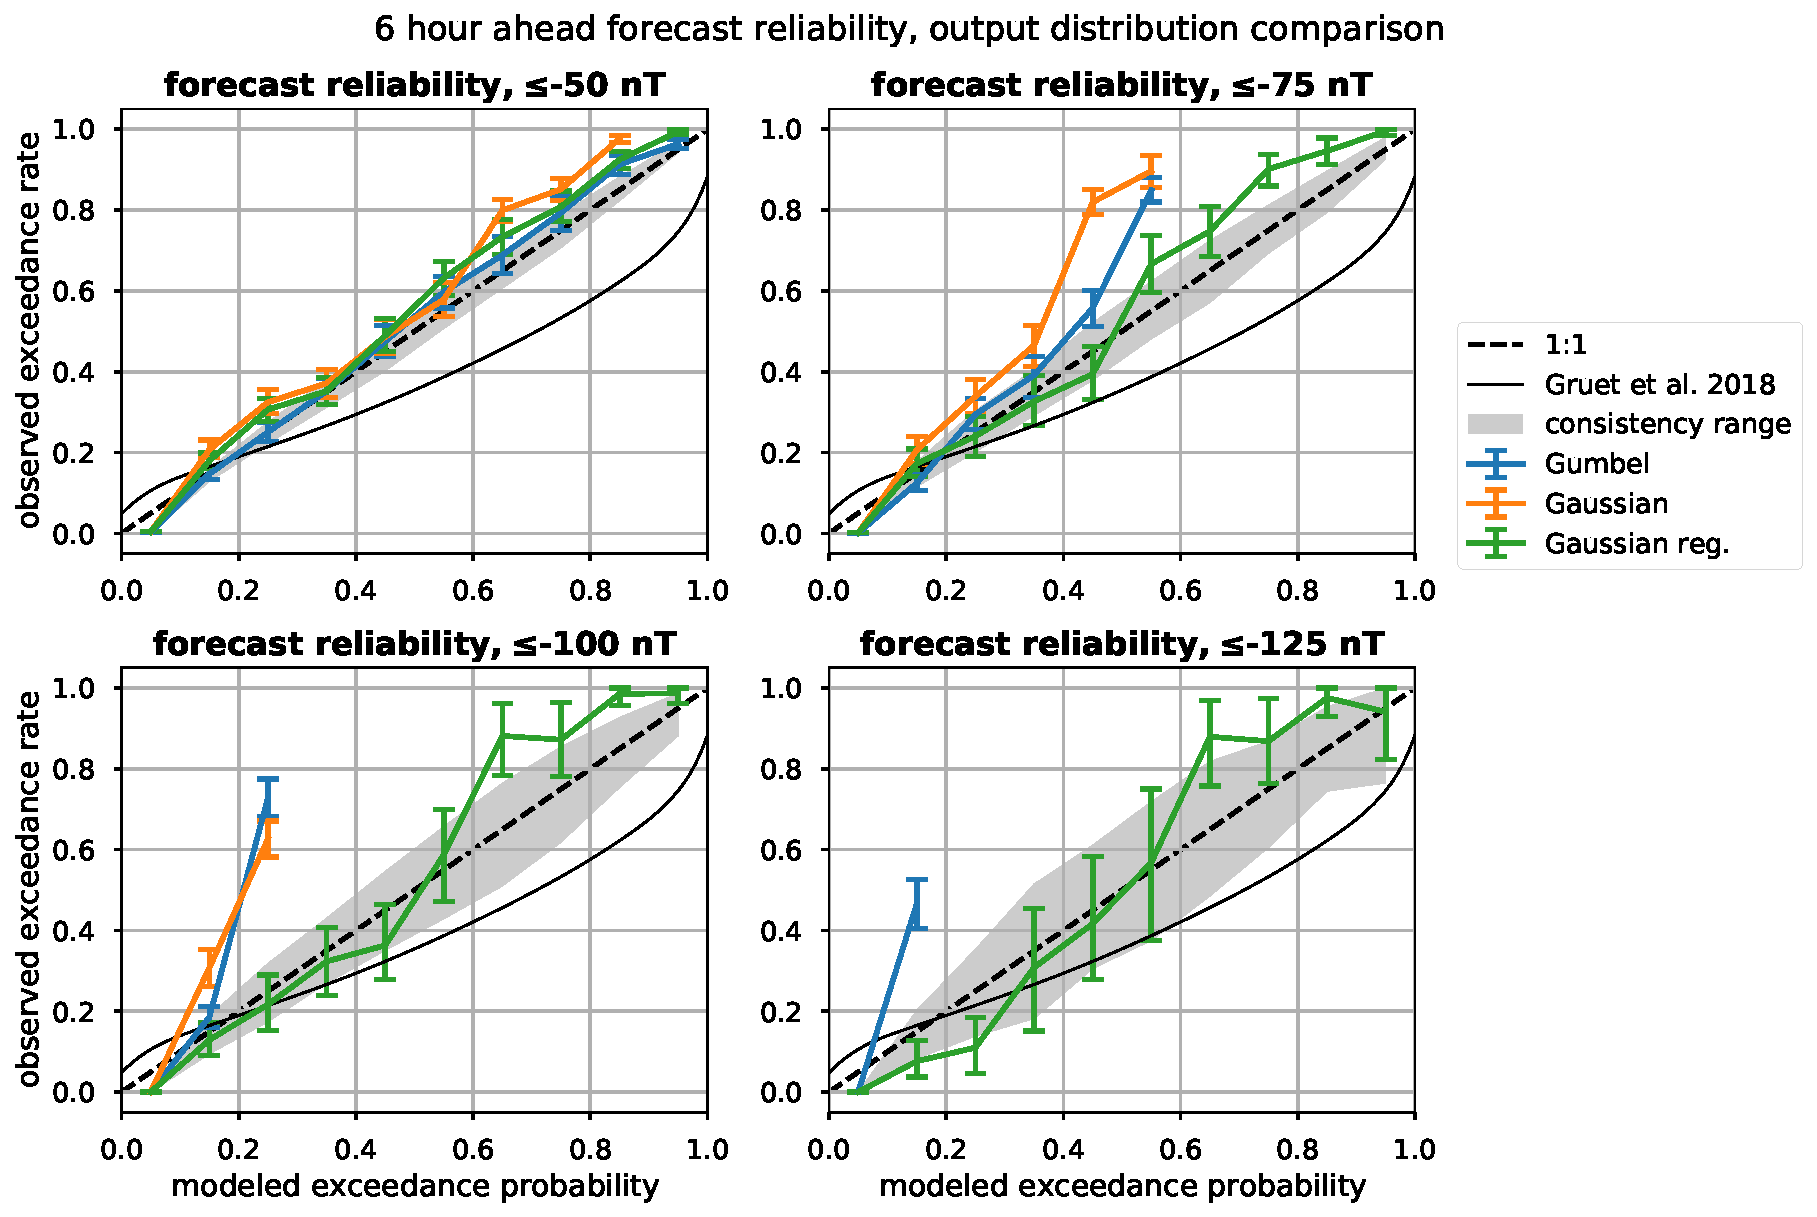
\includegraphics[width=1.0\textwidth]{figures/est_forecast_reliability_distcompare_t+6.pdf} 
  \caption{Reliability curves for the networks with a Gumbel output and cost (blue), Gaussian output and cost (orange), and Gaussian output with regularized cost (green). All curves are for a six hour ahead forecast for four Est thresholds in eleven bins. Exceedance was taken in the negative sense, i.e., taking values less than or equal to the given threshold. Error bars show the 2.5-97.5 percentile range from bootstrapped resampling (number of bootstrapped samples was 1000) within the bins of forecasted exceedance probability. The envelopes show the 2.5-97.5 percentile range from consistency resampling of a perfectly reliable forecast, demonstrating the conceivable range in reliable forecasts given the number of data in each bin \citep{Brocker2007}. The regularized Gaussian network is the most reliable of the three. \added{Also shown is the reliability curve from \cite{Gruet2018} for their six hour ahead Dst forecast, for which the exceedance threshold is unspecified.}}
  \label{fig:reliability}
\end{figure}

While some improvement in forecast reliability for smaller magnitude storms (Est thresholds of -50 and -75~nT) does seem to result from the incorporation of data from the solar disk (Supplement Figure S7), the preceding discussion and the result that forecast behavior does not qualitatively change by adding solar disk inputs (Supplement Text S5) indicates that we are unable to successfully utilize observations from the solar disk to forecast storm arrival and amplitude. This shortcoming suggests that the information necessary for identifying geoeffective solar activity is lacking in the training data, and/or that the network architecture is inadequate for utilizing these data. For instance, the x-ray fluxes are integrated over the entire solar disk, but peaks in these fluxes can often be associated with flare events, which themselves often occur simultaneously with geoeffective mass ejections \citep{Tobiska2013}. Larger, more central flares are associated with larger geomagnetic storms, so adding time series of flare occurrences with locations on the solar disk would complement the input series of x-ray fluxes and CMEs \citep{Tobiska2013}. Futhermore, the CME dataset only includes ejections visible around the rim of the solar disk, while geoeffective ejections occur towards the center. Thus, only centralized ejections that also emit an observable lobe beyond the rim of the solar disk could be reliably associated with geomagnetic storms, potentially rendering the CME database largely irrelevant for the problem of geomagnetic storm forecasting. Finally, integrated solar x-ray flux peaks from flares have been empirically related to solar wind speeds and geomagnetic storm amplitudes, thereby providing a means of learning lag times between solar activity and storm arrivals \citep{Tobiska2013}. However, LSTM networks struggle with learning lag times \citep{Gers2002}, so the network architecture we have utilized is not amenable to this task.  

\section{Conclusions}
% This work has demonstrated a NN architecture capable of learning reliable measures of uncertainty in its forecasts of geomagnetic storms. Learning uncertainty in NN output results in more useful probabilistic forecasts than learning uncertainty in the NN parameters, and the choice of output distribution and cost function has a large impact on the resulting reliability of the trained network. Specifically, adding regularizing terms in the likelihood cost function improves the forecast reliability by incentivizing networks to forecast more reasonable mean values rather than simply increasing forecast uncertainty.

These neural networks are also the first to utilize as inputs observations from the solar disk and L1 point. This provides improved uncertainty forecast and higher reliability, although storm arrival and amplitude forecasting did not substantially improve from the inclusion of these data. Thus, leveraging time series of observations of the solar disk, which are often sparse, remains an open problem, and future network architectures must be carefully designed to utilize these data sources. 
This work has demonstrated a NN architecture capable of learning reliable measures of uncertainty in its forecasts of geomagnetic storms. Learning uncertainty in NN output results in more useful probabilistic forecasts than learning uncertainty in the NN parameters, and the choice of output distribution and cost function has a large impact on the resulting reliability of the trained network. Specifically, adding regularizing terms in the likelihood cost function improves the forecast reliability by incentivizing networks to forecast more reasonable mean values rather than simply increasing forecast uncertainty.

These neural networks \deleted{are also the first to }utilize as inputs observations from \added{both} the solar disk and L1 point\replaced{, slightly improving forecast reliability and skill with respect to networks trained only with L1 inputs. }{. This provides improved uncertainty forecast and higher reliability, although, } \added{However}, storm arrival and amplitude forecasting did not substantially improve from the inclusion of these data. Thus, leveraging time series of observations of the solar disk, which are often sparse, remains an open problem, and future network architectures must be carefully designed to utilize these data sources. 

%%

%  Numbered lines in equations:
%  To add line numbers to lines in equations,
%  \begin{linenomath*}
%  \begin{equation}
%  \end{equation}
%  \end{linenomath*}



%% Enter Figures and Tables near as possible to where they are first mentioned:
%
% DO NOT USE \psfrag or \subfigure commands.
%
% Figure captions go below the figure.
% Table titles go above tables;  other caption information
%  should be placed in last line of the table, using
% \multicolumn2l{$^a$ This is a table note.}
%
%----------------
% EXAMPLE FIGURE
%
% \begin{figure}[h]
% \centering
% when using pdflatex, use pdf file:
% \includegraphics[width=20pc]{figsamp.pdf}
%
% when using dvips, use .eps file:
% \includegraphics[width=20pc]{figsamp.eps}
%
% \caption{Short caption}
% \label{figone}
%  \end{figure}
%
% ---------------
% EXAMPLE TABLE
%
% \begin{table}
% \caption{Time of the Transition Between Phase 1 and Phase 2$^{a}$}
% \centering
% \begin{tabular}{l c}
% \hline
%  Run  & Time (min)  \\
% \hline
%   $l1$  & 260   \\
%   $l2$  & 300   \\
%   $l3$  & 340   \\
%   $h1$  & 270   \\
%   $h2$  & 250   \\
%   $h3$  & 380   \\
%   $r1$  & 370   \\
%   $r2$  & 390   \\
% \hline
% \multicolumn{2}{l}{$^{a}$Footnote text here.}
% \end{tabular}
% \end{table}

%% SIDEWAYS FIGURE and TABLE
% AGU prefers the use of {sidewaystable} over {landscapetable} as it causes fewer problems.
%
% \begin{sidewaysfigure}
% \includegraphics[width=20pc]{figsamp}
% \caption{caption here}
% \label{newfig}
% \end{sidewaysfigure}
%
%  \begin{sidewaystable}
%  \caption{Caption here}
% \label{tab:signif_gap_clos}
%  \begin{tabular}{ccc}
% one&two&three\\
% four&five&six
%  \end{tabular}
%  \end{sidewaystable}

%% If using numbered lines, please surround equations with \begin{linenomath*}...\end{linenomath*}
%\begin{linenomath*}
%\begin{equation}
%y|{f} \sim g(m, \sigma),
%\end{equation}
%\end{linenomath*}

%%% End of body of article

%%%%%%%%%%%%%%%%%%%%%%%%%%%%%%%%
%% Optional Appendix goes here
%
% The \appendix command resets counters and redefines section heads
%
% After typing \appendix
%
%\section{Here Is Appendix Title}
% will show
% A: Here Is Appendix Title
%
%\appendix
%\section{Here is a sample appendix}

%%%%%%%%%%%%%%%%%%%%%%%%%%%%%%%%%%%%%%%%%%%%%%%%%%%%%%%%%%%%%%%%
%
% Optional Glossary, Notation or Acronym section goes here:
%
%%%%%%%%%%%%%%
% Glossary is only allowed in Reviews of Geophysics
%  \begin{glossary}
%  \term{Term}
%   Term Definition here
%  \term{Term}
%   Term Definition here
%  \term{Term}
%   Term Definition here
%  \end{glossary}

%
%%%%%%%%%%%%%%
% Acronyms
%   \begin{acronyms}
%   \acro{Acronym}
%   Definition here
%   \acro{EMOS}
%   Ensemble model output statistics
%   \acro{ECMWF}
%   Centre for Medium-Range Weather Forecasts
%   \end{acronyms}

%
%%%%%%%%%%%%%%
% Notation
%   \begin{notation}
%   \notation{$a+b$} Notation Definition here
%   \notation{$e=mc^2$}
%   Equation in German-born physicist Albert Einstein's theory of special
%  relativity that showed that the increased relativistic mass ($m$) of a
%  body comes from the energy of motion of the body—that is, its kinetic
%  energy ($E$)—divided by the speed of light squared ($c^2$).
%   \end{notation}




%%%%%%%%%%%%%%%%%%%%%%%%%%%%%%%%%%%%%%%%%%%%%%%%%%%%%%%%%%%%%%%%
%
%  ACKNOWLEDGMENTS
%
% The acknowledgments must list:
%
% >>>>	A statement that indicates to the reader where the data
% 	supporting the conclusions can be obtained (for example, in the
% 	references, tables, supporting information, and other databases).
%
% 	All funding sources related to this work from all authors
%
% 	Any real or perceived financial conflicts of interests for any
%	author
%
% 	Other affiliations for any author that may be perceived as
% 	having a conflict of interest with respect to the results of this
% 	paper.
%
%
% It is also the appropriate place to thank colleagues and other contributors.
% AGU does not normally allow dedications.


\acknowledgments
This work was partially supported by the ESA through the Swarm DISC project. The low (hourly) resolution OMNI data were obtained from the GSFC/SPDF OMNIWeb interface (\url{https://omniweb.gsfc.nasa.gov}). We acknowledge use of the LASCO SOHO CME catalog (\url{https://cdaw.gsfc.nasa.gov/CME\_list/}), which is generated and maintained at the CDAW Data Center by NASA and The Catholic University of America in cooperation with the Naval Research Laboratory. SOHO is a project of international cooperation between ESA and NASA. We acknowledge use of GOES mission x-ray flux data, accessed from \url{https://satdat.ngdc.noaa.gov/sem/goes/data/avg/}. Finally, we acknowledge use of the EST-IST-DST dataset from NOAA accessed from \url{https://www.ngdc.noaa.gov/geomag/est\_ist.shtml}. All data and analysis presented in this study are available as Jupyter notebooks at \url{https://doi.org/10.5281/zenodo.3751682}.


%% ------------------------------------------------------------------------ %%
%% References and Citations

%%%%%%%%%%%%%%%%%%%%%%%%%%%%%%%%%%%%%%%%%%%%%%%
% BibTeX is preferred:
%
\bibliography{refs.bib}
%
% no need to specify bibliographystyle
%%%%%%%%%%%%%%%%%%%%%%%%%%%%%%%%%%%%%%%%%%%%%%%



% Please use ONLY \citet and \citep for reference citations.
% DO NOT use other cite commands (e.g., \cite, \citeyear, \nocite, \citealp, etc.).
%% Example \citet and \citep:
%  ...as shown by \citet{Boug10}, \citet{Buiz07}, \citet{Fra10},
%  \citet{Ghel00}, and \citet{Leit74}.

%  ...as shown by \citep{Boug10}, \citep{Buiz07}, \citep{Fra10},
%  \citep{Ghel00, Leit74}.

%  ...has been shown \citep [e.g.,][]{Boug10,Buiz07,Fra10}.


\end{document}



More Information and Advice:

%% ------------------------------------------------------------------------ %%
%
%  SECTION HEADS
%
%% ------------------------------------------------------------------------ %%

% Capitalize the first letter of each word (except for
% prepositions, conjunctions, and articles that are
% three or fewer letters).

% AGU follows standard outline style; therefore, there cannot be a section 1 without
% a section 2, or a section 2.3.1 without a section 2.3.2.
% Please make sure your section numbers are balanced.
% ---------------
% Level 1 head
%
% Use the \section{} command to identify level 1 heads;
% type the appropriate head wording between the curly
% brackets, as shown below.
%
%An example:
%\section{Level 1 Head: Introduction}
%
% ---------------
% Level 2 head
%
% Use the \subsection{} command to identify level 2 heads.
%An example:
%\subsection{Level 2 Head}
%
% ---------------
% Level 3 head
%
% Use the \subsubsection{} command to identify level 3 heads
%An example:
%\subsubsection{Level 3 Head}
%
%---------------
% Level 4 head
%
% Use the \subsubsubsection{} command to identify level 3 heads
% An example:
%\subsubsubsection{Level 4 Head} An example.
%
%% ------------------------------------------------------------------------ %%
%
%  IN-TEXT LISTS
%
%% ------------------------------------------------------------------------ %%
%
% Do not use bulleted lists; enumerated lists are okay.
% \begin{enumerate}
% \item
% \item
% \item
% \end{enumerate}
%
%% ------------------------------------------------------------------------ %%
%
%  EQUATIONS
%
%% ------------------------------------------------------------------------ %%

% Single-line equations are centered.
% Equation arrays will appear left-aligned.

Math coded inside display math mode \[ ...\]
 will not be numbered, e.g.,:
 \[ x^2=y^2 + z^2\]

 Math coded inside \begin{equation} and \end{equation} will
 be automatically numbered, e.g.,:
 \begin{equation}
 x^2=y^2 + z^2
 \end{equation}


% To create multiline equations, use the
% \begin{eqnarray} and \end{eqnarray} environment
% as demonstrated below.
\begin{eqnarray}
  x_{1} & = & (x - x_{0}) \cos \Theta \nonumber \\
        && + (y - y_{0}) \sin \Theta  \nonumber \\
  y_{1} & = & -(x - x_{0}) \sin \Theta \nonumber \\
        && + (y - y_{0}) \cos \Theta.
\end{eqnarray}

%If you don't want an equation number, use the star form:
%\begin{eqnarray*}...\end{eqnarray*}

% Break each line at a sign of operation
% (+, -, etc.) if possible, with the sign of operation
% on the new line.

% Indent second and subsequent lines to align with
% the first character following the equal sign on the
% first line.

% Use an \hspace{} command to insert horizontal space
% into your equation if necessary. Place an appropriate
% unit of measure between the curly braces, e.g.
% \hspace{1in}; you may have to experiment to achieve
% the correct amount of space.


%% ------------------------------------------------------------------------ %%
%
%  EQUATION NUMBERING: COUNTER
%
%% ------------------------------------------------------------------------ %%

% You may change equation numbering by resetting
% the equation counter or by explicitly numbering
% an equation.

% To explicitly number an equation, type \eqnum{}
% (with the desired number between the brackets)
% after the \begin{equation} or \begin{eqnarray}
% command.  The \eqnum{} command will affect only
% the equation it appears with; LaTeX will number
% any equations appearing later in the manuscript
% according to the equation counter.
%

% If you have a multiline equation that needs only
% one equation number, use a \nonumber command in
% front of the double backslashes (\\) as shown in
% the multiline equation above.

% If you are using line numbers, remember to surround
% equations with \begin{linenomath*}...\end{linenomath*}

%  To add line numbers to lines in equations:
%  \begin{linenomath*}
%  \begin{equation}
%  \end{equation}
%  \end{linenomath*}



